\documentclass[11pt]{article}
\usepackage{amsmath}
\usepackage{bm}
\usepackage[margin=1in]{geometry}
\usepackage{url}
\usepackage{hyperref}
\usepackage[numbers,sort&compress, square]{natbib}
\usepackage{graphicx}
\usepackage[T1]{fontenc}
\usepackage[sc]{mathpazo}
\usepackage{pdflscape}
\usepackage{threeparttable}
\usepackage{booktabs}
\linespread{1.5}

\setlength{\parindent}{0pt}
\setlength{\parskip}{2ex plus 1ex minus 1ex}

\begin{document}
\title{A tree-ring based reconstruction of early summer precipitation in southwestern Virginia {(1750-1981)}}
%\author{Andria Dawson\footnote{University of Alberta, Edmonton AB; \url{adawson@ualberta.ca}},\ \ 
%   David Austen\footnote{Appalachian State University},\ \ 
%   David Walker\footnote{Virginia Tech},\ \ 
%   and Valerie Trouet\footnote{University of Arizona}}
\author{Andria Dawson, David Austin, David Walker, and Valerie Trouet}

\maketitle

\section*{Abstract}

In a closed-canopy forest, stand dynamics play an important role in shaping the forest, and it has been hypothesized that dense forests are not sufficiently limited by climate to warrant climate reconstruction. We collected \textit{Quercus prinus} tree-ring data from a dense forest in the Appalachians, and after removal of stand dynamics and age trends we find strong correlations between annual tree growth and early summer precipitation. To strengthen the climate signal, we include additional southeastern US \textit{Quercus prinus} chronologies in a nested principal component analysis (PCA). Correlation between the growth proxy and early summer precipitation was increased through PCA, and assessment of reconstruction skill was favorable. The reconstruction was modeled using a Bayesian regression model, which allowed uncertainty to be quantified. The reconstruction covered the period 1750-1981, and extended the instrumental record by 150 years. The reconstruction showed key drought years identified by others, as well as 11-year periodicity.

%%
%% body
%%

\section{Introduction}

%\nocite{NCDC2012}

The Southern Appalachian region is one of the most biologically diverse
temperate forest systems.  This region has supported continuous forest
communities longer than any other area on the North American continent,
and hosts many rare, endemic species \cite{NCNHP2012}. Additionally,
it harbors many disjunct species populations. The southern
Appalachians also provide ecosystem services such as carbon storage,
watershed and water quality protection, and serve as a timber source
\cite{zipper2011restoring}. In order to protect these valuable resources,
it is crucial that we understand the past climate of this
area and how it has influenced the many ecosystems within the region.
Understanding this past climate-ecosystem relationship will enable scientists and landowners
to better manage natural resources in a our current changing climate.

Global circulation models project an increase in average global surface
temperatures of $1.0-3.5^{\circ}$C by the end of this century due to
continued increases in greenhouse-gas emissions \cite{pachauri2007climate,
kattenberg1996climate}. However the influence of increased radiative
forcing on precipitation regimes is not well understood, and this is
particularly the case for the southeastern United States (US). The
24 models used to make predictions about climate change in the
Intergovernmental Panel on Climate Change Fourth Assessment Report
were not in consensus with respect to drought frequency in this region
\cite{pachauri2007climate, seager2009drought}.  Uncertainty in climate
projections makes it difficult to predict water and power usage. The
ability to do so is crucial because the southeastern US has experienced
substantial increases in population and energy consumption, over the last
decade \cite{seager2009drought, sobolowski2012evaluation}. It is important
that the public and planners in the Southeast have access to information
regarding climate change projections and mitigation. Through the use of
tree-ring based climate reconstructions, we can better understand
past precipitation regimes at both decadal- and centennial time-scales and 
improve projections of future precipitation patterns.% in a changing climate.


In order to reduce uncertainty in climate model projections and to
extend meteorological records further back in time, tree-ring data are
commonly used as regional proxies, particularly in regions where drought
(e.g. the American Southwest, \cite{cook2004long}) or summer temperature
(e.g. the European Alps, \cite{buntgen2007growth}) is the limiting tree
growth factor. However, tree-ring data have also successfully been used
for climate reconstructions in the eastern US \cite{leblanc1993temporal,
stahle1993, cook1999drought}. Traditionally it has been understood that
trees in a closed-canopy forest are not limited by climate to the same
extent as trees growing on the forest border \cite{fritts1976tree}. Within
a dense forest, stand dynamics play an important role in shaping the
forest structure through their influence on radial tree growth and tree
survival. As these interactions between individuals increase in strength,
the climatic influence on tree growth becomes less dominant.

Trees growing in temperate regions characterized by high humidity, such
as those in the Southeast US, are typically thought to be less sensitive
to climate than trees in semiarid regions \cite{phipps1982comments}. This
belief supports the idea that the degree to which an environmental factor
is limiting affects the amount of variability in that factor that is
seen in tree-ring time series.

Despite the challenges of finding a strong climate signal in tree-ring
time series in southeastern US forests, numerous studies have identified
climate-growth correlations \cite{pan1997dendroclimatological,
speer2009climate, rubino2000dendroclimatological}. For example,
\citet{pan1997dendroclimatological} showed that after tree-ring
standardization, both annual ring-width and basal area increments
of four deciduous species in Virginia were positively correlated
with precipitation from both the prior summer, autumn, and current
summer. They also report negative correlations with air temperature
of the current growing season. \citet{speer2009climate}
found similar correlations between precipitation and temperature and
annual tree growth for oak chronologies from closed canopy forests in
the Southern Appalachian Mountains.

In this study, we determine the presence of a significant relationship
between chestnut oak growth series in the eastern US and early summer
precipitation and ascertain the viability of a climatic reconstruction
based on the chestnut oak growth series as proxy data. The annual growth
proxy data was subsequently used to reconstruct early summer precipitation
using Bayesian methods. Finally, we evaluated the reliability of the
reconstruction by comparing it to other verified regional reconstructions.

%% %% methods %%

\section{Materials and Methods} \label{sec:meth}

\subsection{Tree ring data}

The study site was an Upland Oak-Pine forest located on the north
facing slope of Brush Mountain in South-West Virginia  ($37^{\circ}
\ 22.2$' N, $80^{\circ}\ 14.8$' W), with a site elevation of 558 m
(BM in Figure~\ref{fig:map}). This region is classified as either
humid continental or mountain temperate, and characterized by warm,
humid summers and winters that are predominantly cool with intermittent
warm spells. The mean annual precipitation from 1901-2010 at the nearby
Blacksburg weather station was 1073 mm, while the mean annual temperature
was $10.9^{\circ} C$.

The study site supported older chestnut oak (\textit{Quercus
prinus}) trees amongst a canopy of many species, including scarlet
oak (\textit{Quercus coccinea}), northern red oak (\textit{Quercus
rubra}), red maple (\textit{Acer rubrum}), Virginia pine (\textit{Pinus
virginiana}), pitch pine (\textit{Pinus pungens}), and eastern white pine
(\textit{Pinus strobus}). Site access was adjacent to the Appalachian
trail, although the site was selected to minimize human interference. The
steepness of this slope suggested that climate may be a limiting growth
factor, although the closed canopy and stand density suggested that
stand dynamics may also play a significant role in shaping the forest
structure \cite{fritts1976tree}.

We sampled 56 chestnut oak trees and collected two increment cores per
tree. Samples were dried, mounted, and sanded according to standard
procedure \cite{stokes1996introduction}. Crossdating was performed using
reflected light microscopy and the list method, which facilitates the
identification of marker years that signify relatively favorable or
unfavorable growth years in a stand \cite{yamaguchi1991simple}. All
samples were measured using a LINTAB measurement stage with
0.01mm precision, and visual crossdating was checked using COFECHA
\cite{holmes1983computer}. We used inter-series correlation, a measure
of stand-level signal, and mean sensitivity, to select a total of 76
tree-ring series from 53 trees to be used for site chronology development.

Non-climatic age and stand dynamics related trends were removed from
the individual tree-ring series using smoothing splines with a 50 \%
cutoff at 50 years using ARSTAN software \cite{cook1997calculating}. This
method allowed us the flexibility to remove the episodic-like interaction
effects from the time series, while retaining the high-frequency climatic
variability. Note that as with any filtering technique, inevitably some
portion of the climatic signal will be lost through the removal of these
non-climatic trends \cite{cook1981smoothing}. We here assume that the loss
of climatic signal was negligible, and comparison of the detrended time
series with climatic data ultimately determined if the strength of the
remaining signal was sufficient to perform further analyses. The Brush
Mountain site chronology was then developed based on the individually
detrended tree-ring width time series, and will hereafter be referred
to as BM. \label{sym:BM}

%%  Furthermore, serial correlation is common in tree-ring time series, typically due to
%% the availability of stored water or photosynthates. This autocorrelation
%% effectively reduces the number of independent observations, and
%% therefore must be taken into account through either reduction of the
%% effective sample size to ensure that observation independence, or
%% through autoregressive and/or moving average (ARMA)\label{sym:ARMA}
%% modeling \cite{monserud1986time, cook1987decomposition}. All series
%% were checked for autocorrelation to determine if prewhitening via ARMA
%% modeling was necessary, and applied when deemed necessary. 

We also computed the expressed population signal (EPS)\label{sym:EPS}
to measure the common variability in our chronology at an annual
resolution. EPS depends on both signal coherence and annual sample-depth,
and EPS values which fall below a predetermined cutoff (0.85)
indicate that the chronology is not dominated by a coherent signal,
and is therefore deemed less than ideal for climatic reconstructions
\cite{wigley1984average}.


\subsection{Principal component analysis}

Although water access may not be limiting in southeastern US sites,
a large sample size may compensate to help identify the common climate
signals despite site and individual variability. In regions that are
subject to site heterogeneity, where significant climatic variance
cannot be identified for a standard sample size, principal component
analysis can be an effective means to overcome the lack of strength
of climate signal \cite{peters1981principal, anchukaitis2006forward,
jacoby1989reconstructed}. Through the application of principal component
analysis (PCA)\label{sym:PCA}, tree-ring data collected from a network
of regional sites can be combined to reduce site level noise through
the identification of a common climate signal across sites.

%% It is often the case that data from a single closed-canopy site does
%% not show a strong relationship with climate. In this case, data from
%% additional sites may provide some insight into the regional climate
%% signal through the use of principal component analysis (PCA). PCA can
%% help identify common patterns in climate-modulated tree growth between
%% sites and reduce the dimensionality of the data.

Tree-ring data from 8 eastern US \textit{Quercus prinus} sites
were downloaded from the International Tree-Ring Database (ITRDB;
\url{http://www.ncdc.noaa.gov/paleo/treering.html}) and were
considered for inclusion in a PCA analysis. For each of the eight
sites, individual ring-width time series were detrended using a
smoothing spline with 50\% cutoff at 50 years  \cite{cook1981smoothing}, and subsequently used
to develop site chronologies. Chronology reliability for each of the 8
chronologies was assessed based on the mean sensitivity, inter-series
correlation, EPS, and the first-order autocorrelation. Furthermore,
only chronologies which extended back to at least 1845 (the
length of the BM chronology) and significantly correlated with
regional precipitation anomalies (see below) were retained for
further analysis. Four \textit{Quercus} tree-ring chronologies (3
\textit{Quercus prinus} and 1 \textit{Quercus alba}) met these conditions
(Table~\ref{table:chronStats},Fig.~\ref{fig:stackedChrons}), and all
covered the time interval 1845-1981, while some extended further back
in time. To make use of the of the chronology lengths which extended to
years prior to 1845, chronologies were combined with the BM chronology
in a nested singular value decomposition PCA \cite{wold1987principal,
cook2007north}. The first PCA included 5 contributing chronologies that
covered the 1845-1981 time interval, while the second PCA included 3
contributing chronologies that covered the 1750-1981 time interval. In
each PCA, the components with eigenvalues larger than one were retained
for further analysis, and the components explaining the largest amount of
common variance in the tree-ring chronologies were included in a climate
correlation analysis. The PCAs resulted in two potential reconstructions:
one covering the 1845-1981 interval, and one covering the 1750-1981
interval. Each reconstruction has its own set of skill and accuracy
statistics, as described in \ref{cal_ver}. The final reconstruction is
a combination of segments from the two principal components: 1750-1844,
and 1845-1981.

\subsection{Climate data}

Monthly precipitation sum, average temperature, and average Palmer
Drought Severity Index (PDSI) \cite{palmer1965meteorological} averages
were computed from daily measurements at the Blacksburg climate station
($37^{\circ} \ 12$' N, $80^{\circ}\ 24$' W; elevation 634 m; 1901-2006)
and were used in a correlation function analysis with the tree-ring time
series. Pearson's correlation coefficients were calculated for all months
starting in April of the year previous to the growing season through
current December, as well as for various seasons (Apr-June, July-Sep,
Oct-Dec, Jan-Mar) and annual means.

Average May and June precipitation, and average June and July PDSI
showed the strongest correlation between the Blacksburg station
and the BM chronology. These correlations were then used as guidance for a spatial
correlation analysis between the first principal component and a gridded ($0.5^{\circ} \times 0.5^{\circ}$)
monthly climate data set for the period 1901-2006 \cite[CRUTS3.10;
][]{harris2014updated}. Spatial correlations were calculated using the
KNMI explorer \cite[; http://climexp.knmi.nl]{trouet2013knmi}. The grid
point showing the strongest correlation with the principal component tree-growth proxy was then
selected as a target for reconstruction. We highlight that although our reconstruction is determine for a single point, this reconstruction is representative of the climate in the surrounding region as a result of being constructed from a PCA on growth series from sites spatially distributed around this point.

%% %Temperature, precipation, and PDSI compute from instrumental measurements
%% taken from the Blacksburg climate station  were compared to the
%% BM chronology to indentify any significant correlations (Pearson's
%% correlation coefficients). This information was used to guide the
%% comparison between the BM chronology and high-resolution gridded
%% ($0.5^{\circ} \times 0.5^{\circ}$) monthly CRU climate data, which allowed
%% us to compare grid points of locations with higher elevations. Regions of
%% significant correlation were examined using higher resolution CRU data
%% ($2.5^{\circ} \times 2.5^{\circ}$). Cross correlations were computed
%% between the BM time series and each of the monthly series for temperature,
%% precipitation, and PDSI beginning with April of the previous growing
%% season through current December for the $1901 - 1981$ period.

\subsection{Reconstruction methods}

Precipitation was modelled using a Bayesian linear
regression model, with the principal component growth proxy (covering the
period 1750-1981) as a predictor. The precipitation model is written
as 

\begin{align}
\label{eqn1}
y_t &\sim Normal( \mu_t, \sigma^2)\\
\mu_t &= \beta_0 + \beta_1 x_t,
\end{align}
where $y_t$ represents precipitation values for the identified grid cell and $x_t$
is the first principal component value at year $t$. Uninformative
priors were placed on all three parameters as follows: $\beta_i \sim
\text{Normal}(\vec{0},1000)$, and $\sigma^2 \sim \text{Uniform}(0,100)$.
Posterior distributions for all three parameters ($\beta_0$, $\beta_1$,
and $\sigma^2$) were sampled using an adaptive Markov Chain Monte Carlo (MCMC)
algorithm with a Metropolis step method, in which proposal distributions were adjusted 
accordingly when acceptance rates fell outside ideal range of 0.2-0.5. The algorithm was run
run for 100,000 iterations with a burn-in of 50,000. Parameter estimates were thinned so that only every
tenth estimate was saved to disk. The 0.025, 0.5 and 0.975 quantiles
of these estimated were determined to define an upper and lower bound
for a 95\% credible interval, as well as the median. At each iteration,
parameter estimates were used to compute estimated precipitation. A 95\%
predictive interval was computed from these precipitation estimates
using the 0.025, 0.5 and 0.975 quantiles. Note that frequentist methods could have been used with similar results, although we much prefer the simple interpretation of the Bayesian credible interval.

\subsection{Model calibration and verification} \label{cal_ver}

To assess the accuracy of the modeled precipitation anomalies, we used a split-period (1901-1941 and 1941-1981) calibration. Both
the 1901-1940 and 1941-1981 periods of climate data were used in turn as the
calibration period (denoted by $y_t$ in \ref{eqn1}), to determine if the accuracy of the reconstruction
was sufficient to warrant further analysis. Data from the period
not used for calibration served as verification data, and for both
calibration/verification pairs we computed the mean squared error
(MSE), reduction of error (RE) \cite{fritts1976tree}, coefficient of
efficiency (CE) \cite{cook1994spatial}, and the squared correlation
($r^2$) (See the National Research Council report Surface Temperature
Reconstructions for the Last 2,000 Years \cite{national2006surface}
for further details on assessing reconstruction skill). % %Lastly,
% we computed the sign test or Gleichl\"{a}ufigkeit (GLK) score which
% measures the similarity of the relative annual change in value between
% two time series \cite{speer2010fundamentals, schweingruber1988tree}.

\subsection{Reconstruction analysis}

We compared our precipitation reconstruction to six published regional
precipitation and drought reconstructions as external validation
(Table~\ref{table:reconDeets}). One drought reconstruction was obtained
from the North American Drought Atlas (NADA) \cite{cook1999drought} which
is a gridded reconstruction of PDSI values for June through August. The
second drought reconstruction was a July PDSI reconstruction (JT) for
Virginia and North Carolinian coastal regions \cite{stahle1998lost}. The
remaining four reconstructions identified for comparison were
precipitation reconstructions for the North Carolina (NC), South Carolina
(SC), and Georgia (GA) regions for the months of April though June for NC,
and March through June for SC and GA \cite{stahle1992reconstruction},
and one reconstruction for early summer anomalies for the Montpelier
region (MP) \cite{druckenbrod2003late}.

Reconstructions that were significantly correlated with our final
precipitation reconstruction were compared using 31-year windowed
correlation plots, which facilitated the identification of periods of
pattern dissimilarity.

Furthermore, we used a spectral wavelet analysis to
identify dominant cyclical behavior in our reconstruction
\cite{torrence1998practical}. Spectrum values were averaged with 2
frequencies per bin to simplify interpretation.

%% %% results %%

\section{Results}

The BM chronology covered the period 1764-2010 CE, had an
interseries correlation of 0.556 and a mean sensitivity of 0.208
(Table~\ref{table:chronStats}). The EPS was above the 0.85 cutoff for
1845-1981 and thus we used the chronology over this period. A spatial
correlation analysis between considered climate variables and BM identified the grid point $37.5-38^{\circ}$ N.,
$80.5-81^{\circ}$ E. as the location that correlated most highly with our
chronology. The BM chronology was significantly positively correlated with monthly
PDSI values from April of the previous year to December of the current
year (Fig.~\ref{fig:climCorr}B), except for previous May and previous
October. We found particularly strong correlations between BM
and monthly PDSI over the May through August growing season, with the
highest correlation being with average June and July PDSI (jjPDSI;
$r=0.55$, $p<0.01$). Furthermore, we found significant, positive
correlations with precipitation of the previous year June and current
year May and June (Fig.~\ref{fig:climCorr}A). When averaging monthly
precipitation values over the months May and June (mjPR), correlation
increased to $r=0.5$ ($p<0.01$). The BM chronology did not correlate
with monthly temperature values (Fig.~\ref{fig:climCorr}C).

Based on this climate-growth analysis, mjPR and jjPDSI were considered
as candidate targets for reconstruction. An assessment of the
calibration/verification statistics for a reconstruction based on the BM
chronology alone (results not shown), however, suggested that the climate
signal was not sufficient to warrant adequate reconstruction skill. We
therefore combined the BM chronology with four existing oak chronologies
from nearby sites (Fig.~\ref{fig:map}, \ref{fig:stackedChrons}) in a
nested PCA approach. All four chronologies were significantly positively
correlated with the mjPR and jjPDSI values from the monthly data set
obtained from the spatial correlation analysis. 

The first PC axis (PC1) of a PCA performed on all five chronologies
for the period of overlap 1845-1981 explained 57.0\% of the common
variance, while the second axis explained 15.2\%. All oak chronologies had
the same sign on PC1, thus emphasizing the correspondence between the
time series. We then performed another PCA including only the three
chronologies which extended back to the year 1750 (LH, WD, OC). PC1
over this longer period explained 56.0\% of the common variance and
PC2 explained 28.3\%. We then merged the PC1 time series of the two PC
analyses (which were strongly positively correlated; $r=0.93$, $p <
0.01$) at the year 1845 (PCA2: 1750-1844, PCA1: 1845-1981) to form a
single chronology extending from 1750 to 1981. This chronology will from
hereon be named SWV (for southwest Virginia).

When comparing SWV with monthly climate variables, we generally find
higher correlations than for the individually contributing tree-ring
series (Fig.~\ref{fig:climCorr}) and
this is particularly true for mjPR ($r=0.61$, $p<0.01$) and jjPDSI
($r=0.63$, $p<0.01$). We thus tested mjPR and jjPDSI as potential
reconstruction targets in a split calibration/verification scheme
(\cite{fritts1990methods}; Table~\ref{table:reconStats}). RE and CE
values were negative for jjPDSI when using the later calibration period
(1942-1981), indicating a poor fit of the reconstruction model. RE and
CE are key statistics to determine the skill of a reconstruction, and
our decision to reconstruct mjPR rather than jjPDSI was based on these
values. Our final mjPR reconstruction, now referred to as rSWV, was calibrated against the entire
1901-1981 interval. Estimates of rSWV and corresponding 95\% predictive intervals were computed for each year of the period of reconstruction using posterior parameter draws (Fig.~\ref{fig:precipRecon}.

We compared rSWV to other regional moisture reconstructions (Table~\ref{table:reconComps})
and found positive correlations across the board. The strongest
correlation was found with the NADA summer drought reconstruction
($r=0.53$, $p<0.01$), although we note that the LH chronology was used
in the construction of both rSWV and NADA which implies that these
records are not completely independent. A spectral analysis shows a
periodicity in the rSWV reconstruction, with peaks at 11, 17, and 24 years
(Fig.~\ref{fig:spectral}).

%% %% discussion %%

\section{Discussion}

We investigated the relationship between climate and annual radial growth
of chestnut oak growing at a closed canopy site in the southeastern
US. After removing the portion of the signal attributed to stand dynamics
and intrinsic age trends, we found that early summer (May through June)
moisture was the strongest, positive influence on radial growth. Similar
climate-growth relationships have been identified by previous studies on
oak in the southeastern US \cite{speer2009climate, li2011dendroclimatic}
and can be explained by ecophysiological mechanisms. 
%%, Estes 1970; Blasing and Duvick 1984; Jacobi and Tainter 1988; Graumlich 1993; Tardif
%%et al. 2006. 
 Radial growth of oak species typically starts in April or
May after leaf-out, and even in years with adequate moisture, is 90\%
complete by the end of July \cite{robertson1992factors}. In the first
months of the growing season, carbon is allocated predominantly to radial
thickening, while later in the season the focus of this allocation is
shifted to carbohydrate storage \cite{zweifel2006intra}. Under severe
moisture stress, oak carbon allocation is shifted from shoot to root,
thereby increasing the root/shoot ratio \cite{dickson1996oak}. Chestnut
oak is considered to be more tolerant to drought stress than other oak
species and exhibits several morphological adaptations in order to better
cope with moisture stress events \cite{dickson1996oak}. However, we found
that its radial growth was strongly influenced by moisture availability,
suggesting that in years with inadequate moisture, radial growth is not
a priority and carbon allocation is likely focused on maintenance or
root development. The identifiable moisture-response in the detrended
BM chronology demonstrates that oaks in a closed-canopy forest can
indeed be used as paleoclimate proxies, if the non-climatic portion
of the low-frequency signal in the tree-ring time series is removed
with great care \cite{cook1985time, cook1990tree}. The development of
a biologically motivated trend removal algorithm may improve current
practices in dendroclimatology \cite{melvin2008signal}. In addition,
care must be taken in closed canopy forests when attempting to use
growth series as proxy records as younger stands in the stem-exclusion
phase may be dominated by the effects of competition rather than of
climate\cite{oliver1980forest}.

To isolate and strengthen the moisture-growth relationship of the BM
chronology, we performed a nested PCA including five regional summer
moisture sensitive \textit{Quercus} chronologies. The spatial pattern of
the relationship between the resulting SWV chronology and early summer
precipitation \ref{fig:precipCorrMap} indicates that SWV is positively
correlated with moisture in the Great Appalachian Valley. Mountains
play an important role in the hydrological cycle for several reasons,
one of which being that they are the points of origin of most rivers
\cite{beniston1997climatic}. Increases in precipitation in mountainous
regions leads to increased stream flow volumes and surface runoff,
which in turn increases soil moisture in the Appalachian watershed.

Our reconstruction generally shows similar variability as other
reconstructions of moisture variability in the southeastern US
(Table~\ref{table:reconComps}), in particular with a regional
reconstruction of summer PDSI (Figure~\ref{fig:reconCompare}). The
strongest similarity was found with the NADA PDSI Cook reconstruction,
although we note the lack of full independence between these two
records. Despite the overall strong agreement between both records,
a 31-year windowed correlation between rSWV and NADA PDSI indicated that
these records were not consistent for the period 1853-1866.

All five chronologies contributing to SWV show a pattern of reduced
correlation with the NADA PDSI reconstruction during this period,
which coincides with a La Ni\~{n}a event which occurred from
1855-1863 \cite{cole2002multiyear}. La Ni\~{n}a events typically have
stronger impacts on the West Coast, but can also have effects on weather
patterns throughout North America, and have even been shown to affect the
Atlantic hurricane season \cite{pielke1999nina}. During this large-scale
ocean-atmosphere phenomenon, abnormal temperatures increases in the
southeastern US in combination with low moisture availability likely led
to a change in the otherwise stationary precipitation-growth relationship.

The rSWV reconstruction showed anomalies consistent with the instrumental
precipitation record for 1901-1981 \ref{fig:climCorr}. In particular,
the reconstruction correctly identifies the severe nation-wide dust bowl
era drought in the 1930s as well as the drought year 1956, the single
worst drought year of the 1950s drought \cite{fye2003paleoclimatic}. In
years prior to the instrumental record, the SWV reconstruction identifies
several dry periods: 1760-1776, 1867-1874, and 1894-1902.


%% %Other notable corresponding years of low early summer precipitation
%% are 1911, 1914, and 1925. We also note the agreement of extreme
%% precipitation in the years 1928, 1942, and 1950, where documented
%% flooding occurred in the southeastern US \cite{FIXME}. All of the
%% late-spring/early-summer anomalies have been observed across the
%% southeastern US in instrumental records, except for the dry spell
%% in the 1970s \cite{edwards1997characteristics}. In years prior to
%% the instrumental record, the SWV reconstruction identifies several
%% dry periods, most of which have been observed in other moisture
%% reconstructions for the US \cite{FIXME}.


%%  %This shift in moisture limited growth to temperature limited growth
%%  suggests that oaks may

%% %Cole et al., 2002; Cook et al., 2004; %Herweijer et al., 2006; Hoerling
%% and Kumar, 2003; %Schubert et al., 2004; Seager et al., 2005]

The rSWV reconstruction shows an 11-year cyclicity
(\ref{fig:spectral}), a periodicity that has been observed in both
instrumental and paleo-reconstructed temperature and moisture indices,
such as the Northern Hemisphere annual average land air temperature
record extending from 1951-1980, the Northen Hemisphere annual temperature
anomalies reconstructed from proxy data for 1579 1880, as well as for many
of the contiguous states using state-averaged instrumental temperature and
precipitation records \cite{hancock1979cross, lassen1995variability}. In
particular, this cyclic pattern has been identified in June precipitation
in the south-eastern US \cite{hancock1979cross}, but was not apparent in
western US tree-ring based PDSI reconstructions \cite{cook1997new}. This
observed 11-year periodicity is a characteristic of the solar cycle, which
has been shown to be reflected in terrestrial climate, and identified
as one of the contributing factors that determine global temperature
\cite{reid2002solar, national1994Solar, lassen1995variability}. Solar
periods of high and low activity can be measured by the number of sunspots
or the solar cycle length \cite{friis1991length, usoskin2003millennium}. A
larger number of sunspots indicates greater solar activity, and the
magnetic fields in these sunspots have the ability to release large amount
of stored energy as solar flares or coronal mass ejections. These changes
in released energy in turn affect the realized weather patterns.  Studies
have shown that these changes in released energy may also influence
hydroclimate \cite{nichols2012hydroclimate, hancock1979cross}. However,
despite the presence of strong correlations between terrestrial climate
records and solar cycles, physical mechanisms which explain the effects
of external solar forcing on global circulation patterns have yet to be
fully understood \cite{franks2002assessing}.

In conclusion, we have shown that the growth of chestnut oak in
the southern Appalachians is positively influenced by early summer
precipitation. This appears to be a regional trend, as the growth
of several other oak chronologies was strongly associated with our
chronology. We also successfully reconstructed May-June precipitation
for 150 years prior to the instrumental record (1750-1981). Extending
the climate record will allow scientists to have more information as to
how climate affects tree growth and shapes ecosystems. This will better
prepare us for predicting future vegetation changes that may occur with
a changing climate.

\section{Acknowledgements} The authors would like to thank the North American Dendroecological Fieldweek (NADEF) Dendroclimatology group for assisting with data collection, and Carolyn Copenheaver for assisting
with site selection. We would also like to thank the organizers of NADEF, especially Jim Speer.



%%
%% tables and figures
%%

\clearpage
\newpage
%tables
\begin{landscape}
\begin{table}
\begin{center}
\begin{tabular}{ccccrccc} \toprule
Chron & Lat (N), Long (W) & SIC   & MS    & \# Series & MSL & Period      & Citation\\ \midrule
BM    &  37.37, 80.24 & 0.556 & 0.208 & 76        & 128.3              & 1764 - 2010 &         \\
LH    &  35.62, 85.43 & 0.609 & 0.171 & 19        & 181.4              & 1750 - 1997 &  Stahle, D.W.           \\
      &               &       &       &           &                    &             &  \& Therrell, M.D. 2005 \\
WD    &  38.50, 78.35 & 0.523 & 0.163 & 26        & 250.8              & 1642 - 1981 &  Cook, E.R. 1994  \\
CC    &  37.35, 80.37 & 0.592 & 0.218 & 20        & 194.1              & 1722 - 2001 &  Copenheaver, C.A. 2010 \\
OC    &  39.88, 76.40 & 0.575 & 0.169 & 18        & 260.2              & 1631 - 1981 &  Cook, E.R. 1994  \\
%CH    &  38.00, 78.42 & 0.569 & 0.189 & 41        & 69.3               & 1881 - 1993 &  Lawrence, D.M. 1996 \\ 
\bottomrule
\end{tabular}
\end{center}
\caption{Site-specific details for the Brush Mountain (BM), Lynn Hollow, Watchdog Mountain (WD), Craig Creek (CC), and Otter Creek (CC) sites, including location, series intercorrelation (SIC), mean sensitivity (MS), number of series (\# Series), mean series length (MSL), and the data citation. }
\label{table:chronStats}
\vspace{2cm}
\end{table}
\end{landscape}

\begin{table}
\begin{center}
\begin{tabular}{ccc} \toprule
 & \multicolumn{2}{c}{Climate covariate} \\
Proxy & mjPR & jjPDSI \\ \midrule
BM    & 0.50  & 0.55  \\
LH    & 0.55  & 0.48  \\
WD    & 0.43  & 0.59  \\   
CC    & 0.38  & 0.50  \\
OC    & 0.24* & 0.19** \\
%CH    & 0.49  & 0.43  \\
PC1   & 0.61  & 0.63 \\ \bottomrule
\end{tabular}
\caption{Correlations between the growth proxies (site chronologies and first principal component PC1) with both the averaged May-June precipitation (mjPR) and averaged June-July PDSI (jjPDSI). All correlation statistics were significant at the $p<0.01$ level except the correlations indicated by *, which was significant at the $p<0.05$ level, and **, which was not significant ($p=0.09$).}
\end{center}
\label{table:moistureCorrs}
\vspace{2cm}
\end{table}

\begin{table}
\begin{center}
\begin{tabular}{ccccc}
\toprule
 & \multicolumn{4}{c}{Calibration} \\ \cmidrule(lr){2-5}
 & \multicolumn{2}{c}{mjPR} & \multicolumn{2}{c}{jjPDSI} \\ \cmidrule(lr){2-3} \cmidrule(lr){4-5} 
 & 1901-1941 & 1942-1981 & 1901-1941 & 1942-1981\\ \midrule
%MSE & 25927 & 24239 & 85.5 & 151.7 \\ 
RE                 & 0.10 & 0.30 & 0.44 & -0.41 \\
CE                 & 0.10 & 0.30 & 0.39 & -0.60\\
Calibration $R^2$  & 0.64 & 0.56 & 0.58 & 0.74\\
Verification $R^2$ & 0.56 & 0.64 & 0.74 & 0.59 \\
GLK                & 0.55 & 0.79 & 0.68 & 0.64\\ \bottomrule
\end{tabular}
\end{center}
\caption{Reconstruction accuracy statistics for mjPR and jjPDSI. Statistics include the reduction of error (RE), coefficient of efficiency (CE), calibration and verification period $R^2$, and the Gleichl\"{a}ufigkeit (GLK).}
\label{table:reconStats}
\vspace{2cm}
\end{table}

\begin{table}
\begin{center}
\begin{tabular}{cccl} \toprule
Parameter & Mean   & Median & 95\% Credible Interval \\ \midrule
$\beta_0$ & 102.73 & 102.72       & $(98.51, 107.21)$ \\
$\beta_1$ & 67.73  & 68.02        &  $(51.65, 83.66)$\\
$\sigma$  & 23.19  & 23.07        & $(20.28, 26.40)$   \\  \bottomrule
\end{tabular}
\end{center}
\caption{Posterior parameter mean, median, and 95\% credible interval for the intercept ($\beta_0$), slope ($\beta_1$) and standard deviation ($\sigma$) in the linear model which describes average May-June precipitation as a function of the first principal component growth proxy.}
\label{table:mcmcResults}
\vspace{2cm}
\end{table}


\begin{table}
  \begin{center}
    \begin{threeparttable}[b]
      \begin{tabular}{cccccccc}
\toprule
 & \textbf{Recon} & \multicolumn{2}{c}{PDSI} & \multicolumn{4}{c}{Precip} \\ \cmidrule(lr){2-2} \cmidrule(lr){3-4} \cmidrule(lr){5-8}
      & mjPR & JT & NADA & NC & SC & GA & MP\tnote{A} \\  \midrule
mjPR  &  1      & & & & & & \\
JT    &  0.215  & 1     &       &        &        &        &   \\ 
NADA  &  0.593  & 0.502 & 1     &        &        &        &   \\ 
NC    &  0.227  & 0.396 & 0.424 & 1      &        &        &   \\ 
SC    &  0.118* & 0.178 & 0.352 & 0.581  &  1     &        &   \\ 
GA    &  0.079* & 0.196 & 0.345 & 0.474  & 0.766  & 1      &   \\ 
MP    &  0.378  & 0.288 & 0.499 & 0.132* & 0.090* & 0.109* & 1 \\ \bottomrule
      \end{tabular}
      \begin{tablenotes}
      \item [A] Reconstruction covers only the period 1764 - 1966.
      \end{tablenotes}
    \end{threeparttable}
  \end{center}
      \caption{Correlation between the mjPR reconstruction and other reconstructions including the NADA and JT drought reconstructions; and the NC, SC, GA and MP precipitation reconstructions. All values shown were significantly correlated at the $p<0.01$ level, except for those indicated by $^*$ which were not significant.}
  \label{table:reconComps1}
  \vspace{2cm}
\end{table}

\begin{landscape}
\begin{table}
  \begin{center}
    \begin{threeparttable}[b]
      \begin{tabular}{cccccc}
\toprule
Site & Location & Variable & Range   & Data type & Variance           \\
     &       &          & (years) &           & explained ($R^2$)$^A$  \\ \midrule
NADA \cite{cook1999drought}          & 37$^{\circ}$30' N, 80$^{\circ}$0' W   & Jun-Aug PDSI   & 1185-2006 & Tree-rings  & 0.55* \\  
                                     & VA                                    &                &           &             &       \\    
JC   \cite{stahle1998lost}           & Coastal NC and VA                     & July PHDI      & 1700-1984 & Tree-rings  & 0.44 \\ 
NC   \cite{stahle1992reconstruction} & Statewide NC                          & Apr-Jun precip & 933-1985  & Tree-rings  & 0.54 \\
SC   \cite{stahle1992reconstruction} & Statewide SC                          & Mar-Jun precip & 1005-1985 & Tree-rings  & 0.58 \\
GA   \cite{stahle1992reconstruction} & Statewide GA                          & Mar-Jun precip & 933-1985  & Tree-rings  & 0.68 \\
MP   \cite{druckenbrod2003late}      & 38$^{\circ}$13' N, 78$^{\circ}$10' W; & Early summer   & 1784-1966 & Tree-rings; & 0.39 \\ 
                                     & VA                                    & precip         &           & Meteorological diary \\ \bottomrule
      \end{tabular}
      \begin{tablenotes}
      \item [A] $R^2$ values as reported in cited references; may or may not be adjusted.
      \item [*] Median value of $R^2$ for all gridpoints.
      \end{tablenotes}
    \end{threeparttable}
  \end{center}
      \caption{Details for the six southeastern US moisture reconstructions compared to the mjPR reconstruction.}
  \label{table:reconDeets}
  \vspace{2cm}
\end{table}

\begin{table}
  \begin{center}
    \begin{tabular}{cccccc}
\toprule
Years     & Moisture & Consistent with \\ \midrule
1894-1902 & Low & \cite{warrick1980drought, ruffner1998relating, droughtCali}\\
1867-1874 & Low & \cite{droughtCali}\\
1839      & Low & \\
1819      & Low & \cite{lawson2005desert}\\
1772-1777 & Low \\ \bottomrule
      \end{tabular}
  \end{center}
      \caption{Periods of low moisture availability identified by the mjPR reconstruction and documented sources that corroborate this moisture deficit.}
  \label{table:anoms}
  \vspace{2cm}
\end{table}
\end{landscape}



\clearpage
\newpage
%\begin{figure}
%\centering
%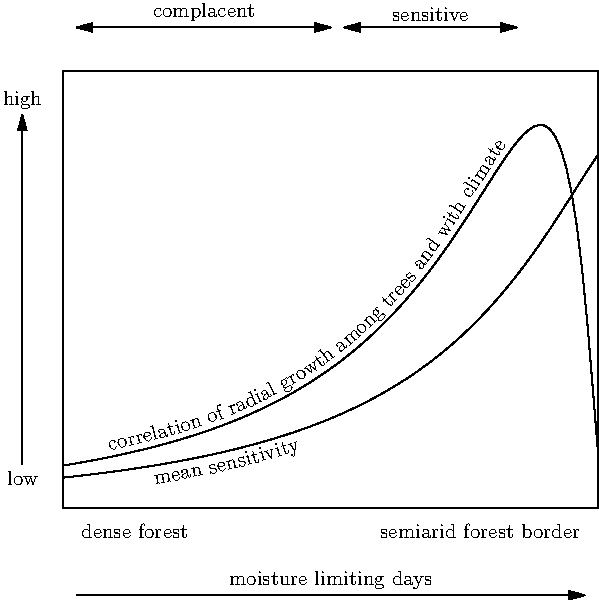
\includegraphics[width=6in]{figures/fritts.pdf}
%\caption{A simplified rendition of the diagram originally seen in \cite{fritts1976tree}.}
%\label{fig:fritts}
%\end{figure}

\begin{figure}
\centering
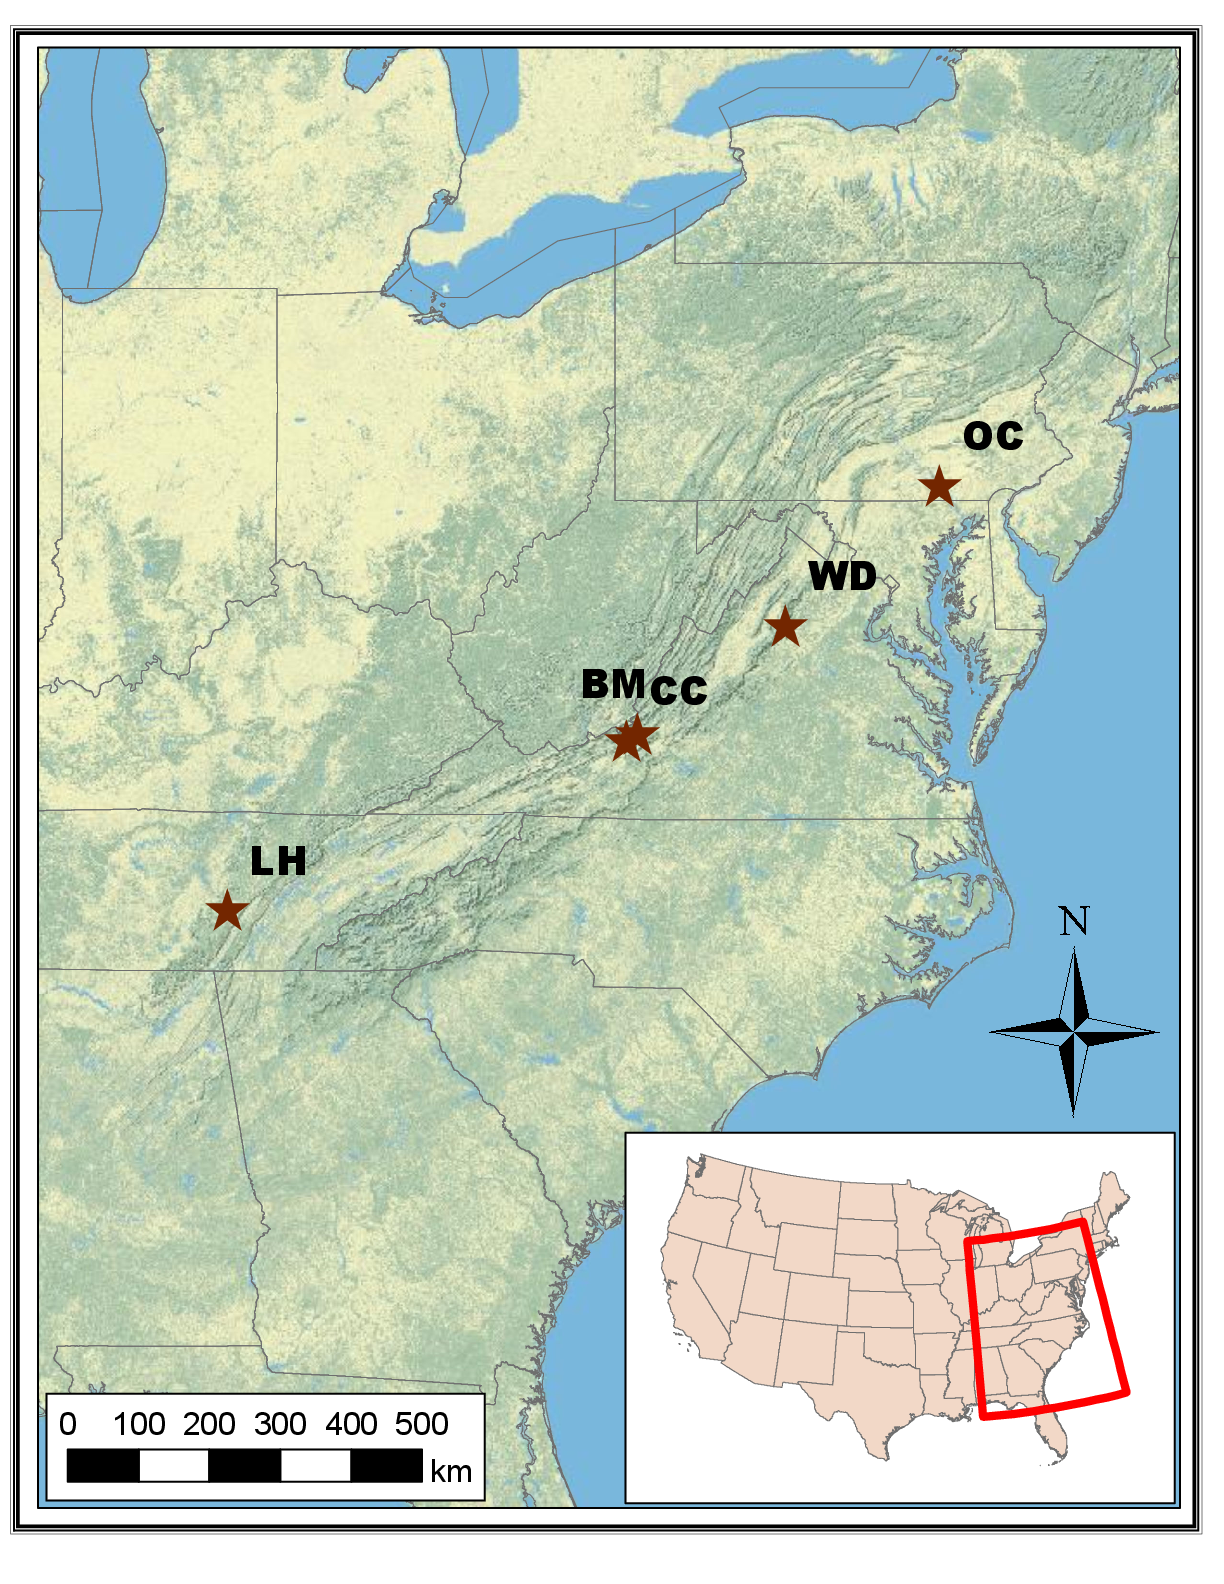
\includegraphics[width=5in]{figures/NewClimateNADEF.png}
\caption{Regional chronology sample locations.}
\label{fig:map}
\end{figure}

\begin{figure}
\centering
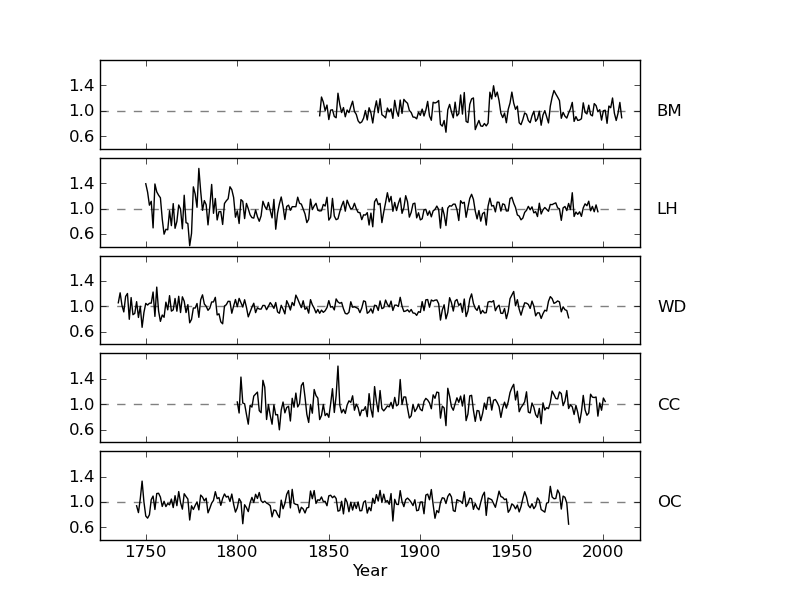
\includegraphics[width=5in]{figures/stacked_chrons.png}
\caption{Plots of the five chronologies used in the principal component analysis. The top panel shows the chronology built from the sample data at Brush Mountain (BM), while the others are the regional chronologies from Lynn Hollow (LH), watchdog Mountain (WD), Craig Creek (CC), and Otter Creek (OC).}
\label{fig:stackedChrons}
\end{figure}

\begin{figure}
\centering
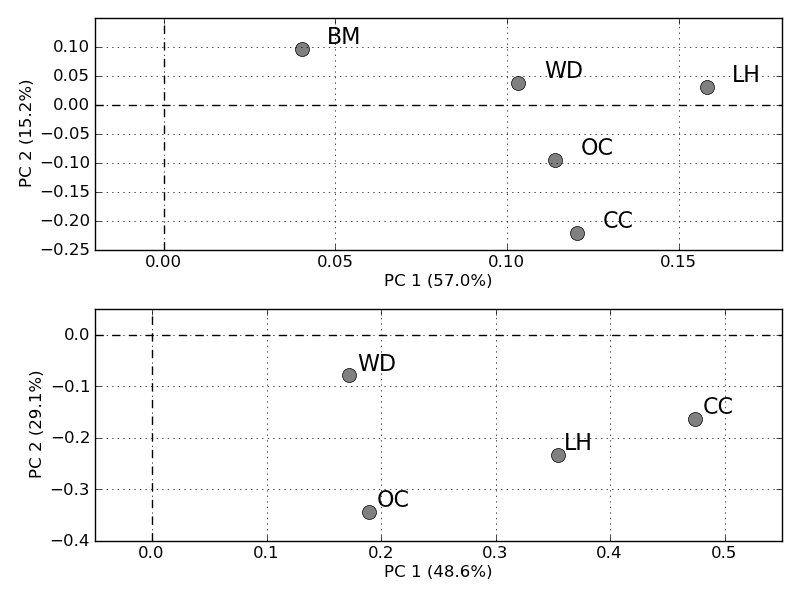
\includegraphics[width=5in]{figures/scoresPlot.png}
\caption{Top: Scatter plot of the loadings for the five chronologies analyzed in the first PCA which covered the period 1845-1981. Bottom: Scatter plot of the loadings for the five chronologies analyzed in the second PCA which covered the period 1750-1981.}
\label{fig:scores}
\end{figure}

\begin{figure}
\centering
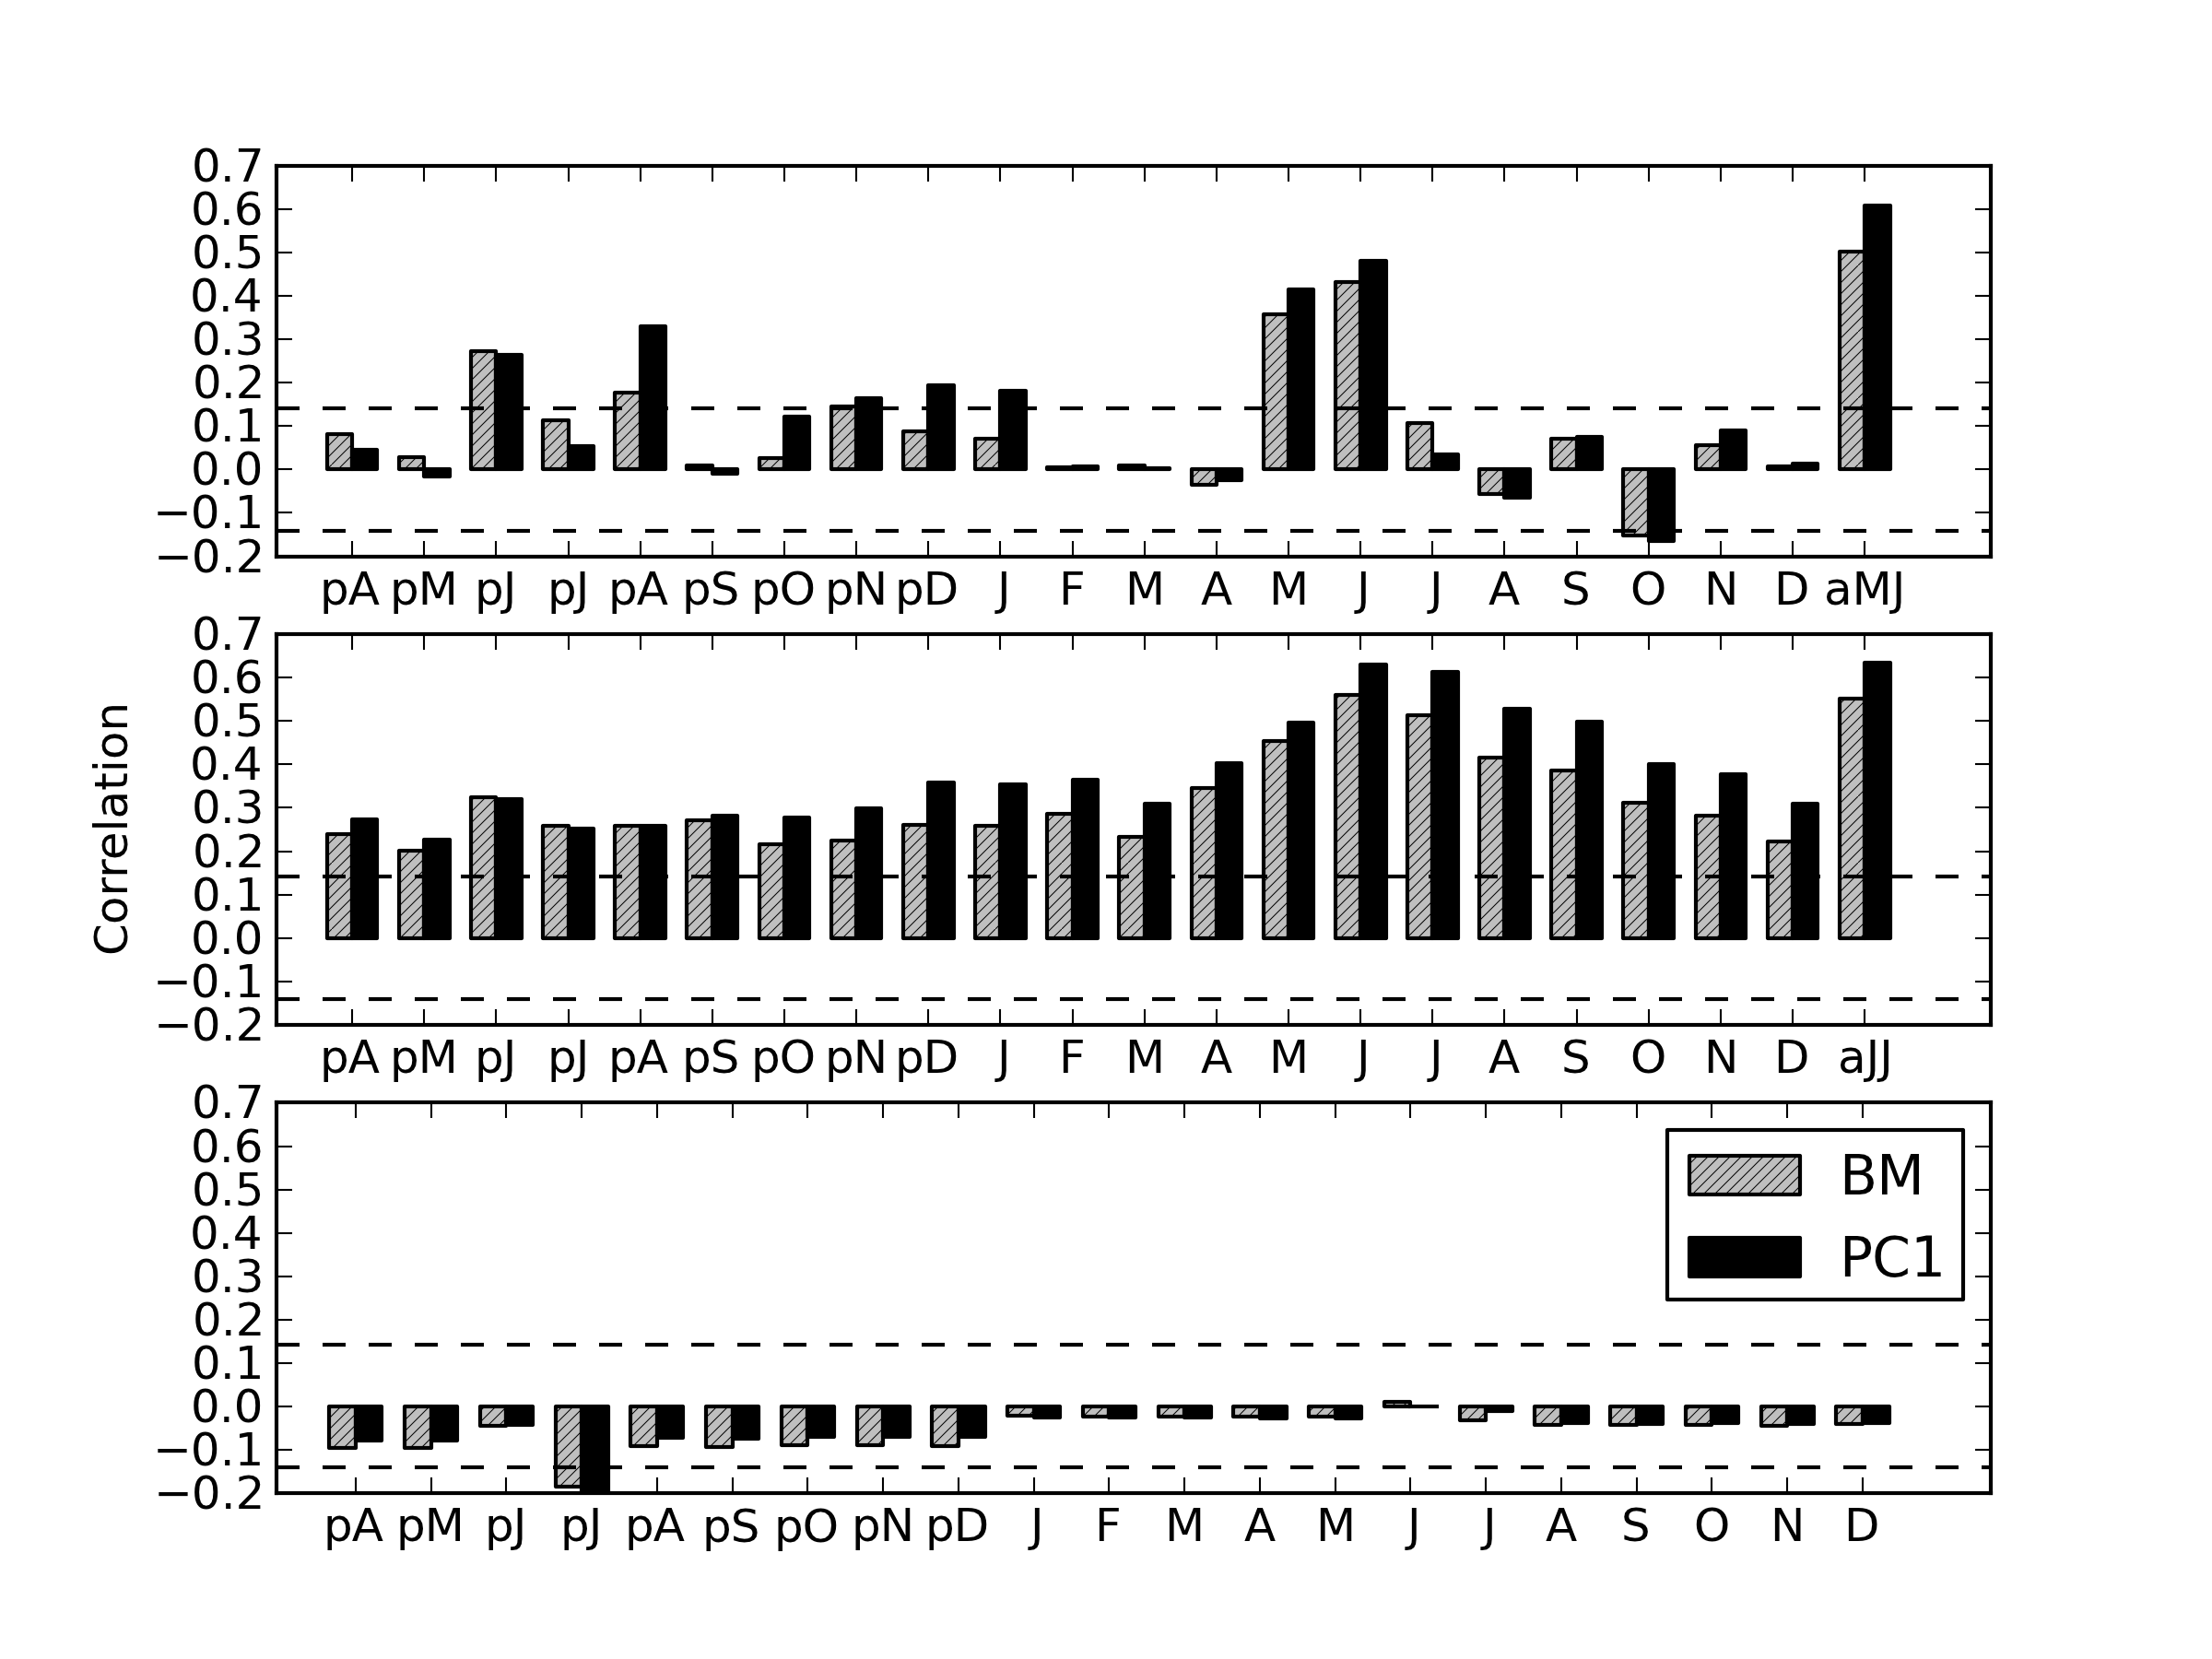
\includegraphics[width=5in]{figures/climCorr.png}
\caption{Top: Correlation between the growth proxies (BM or PC1) and the monthly precipitation from previous April (pA) through December (D) as well as for average May and June (aMJ). Middle: Correlation between the growth proxies (BM or PC1) and average PDSI from previous April (pA) through December (D) as well as for average June and July (aJJ). Bottom: Correlation between the growth proxies (BM or PC1) and average monthly temperature from previous April (pA) through December (D).}
\label{fig:climCorr}
\end{figure}

%\begin{figure}
%\centering
%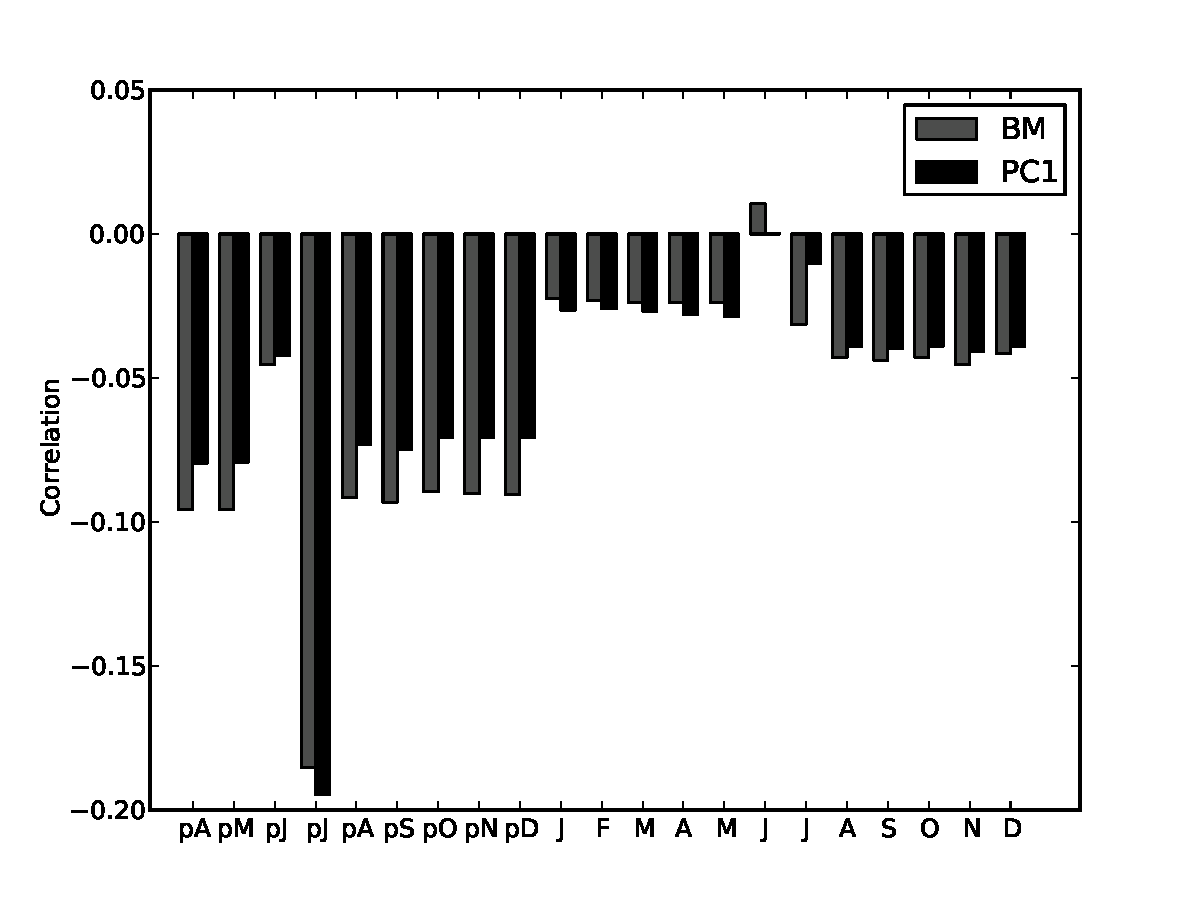
\includegraphics[width=6in]{figures/climCorrTemp.pdf}
%\caption{Correlation between the growth proxies (BM or PC1) and average monthly temperature from previous April (pA) through December (D).}
%\label{fig:tempBarCorr}
%\end{figure}

%\begin{figure}
%\centering
%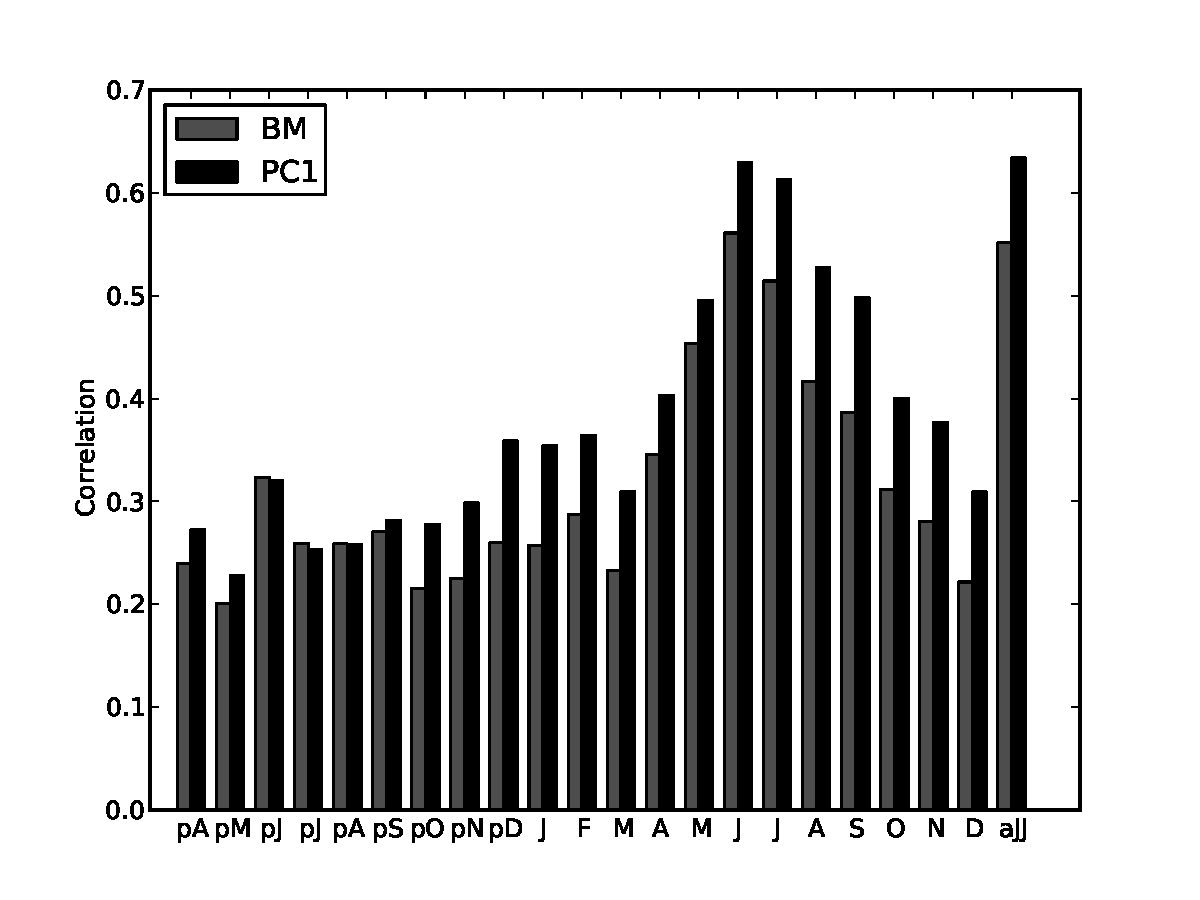
\includegraphics[width=6in]{figures/climCorrPdsi.pdf}
%\caption{Correlation between the growth proxies (BM or PC1) and average PDSI from previous April (pA) through December (D) as well as for averaged June and July (aJJ).}
%\label{fig:pdsiBarCorr}
%\end{figure}

\begin{figure}
\centering
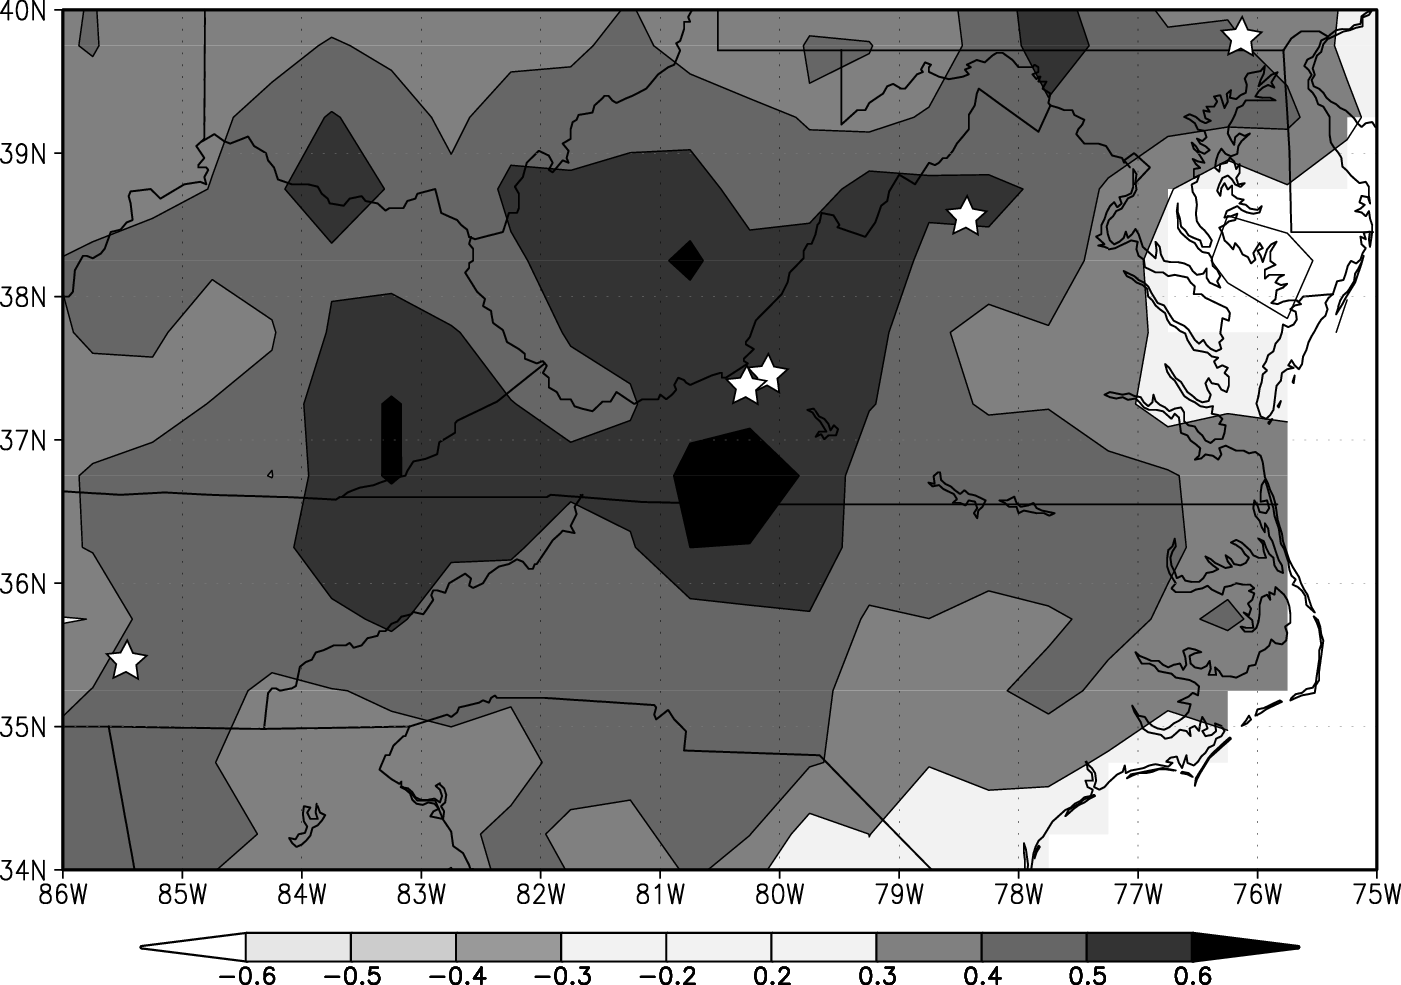
\includegraphics[width=5in]{figures/corrMapPrecipMJ_bw_annot.png}
\caption{Correlation map showing the correlation between the first principal component and averaged May-June precipitation. Stars indicate the locations of the sites where the tree-rings used to develop the contributing chronologies were sampled.}
\label{fig:precipCorrMap}
\end{figure}

%\begin{figure}
%\centering
%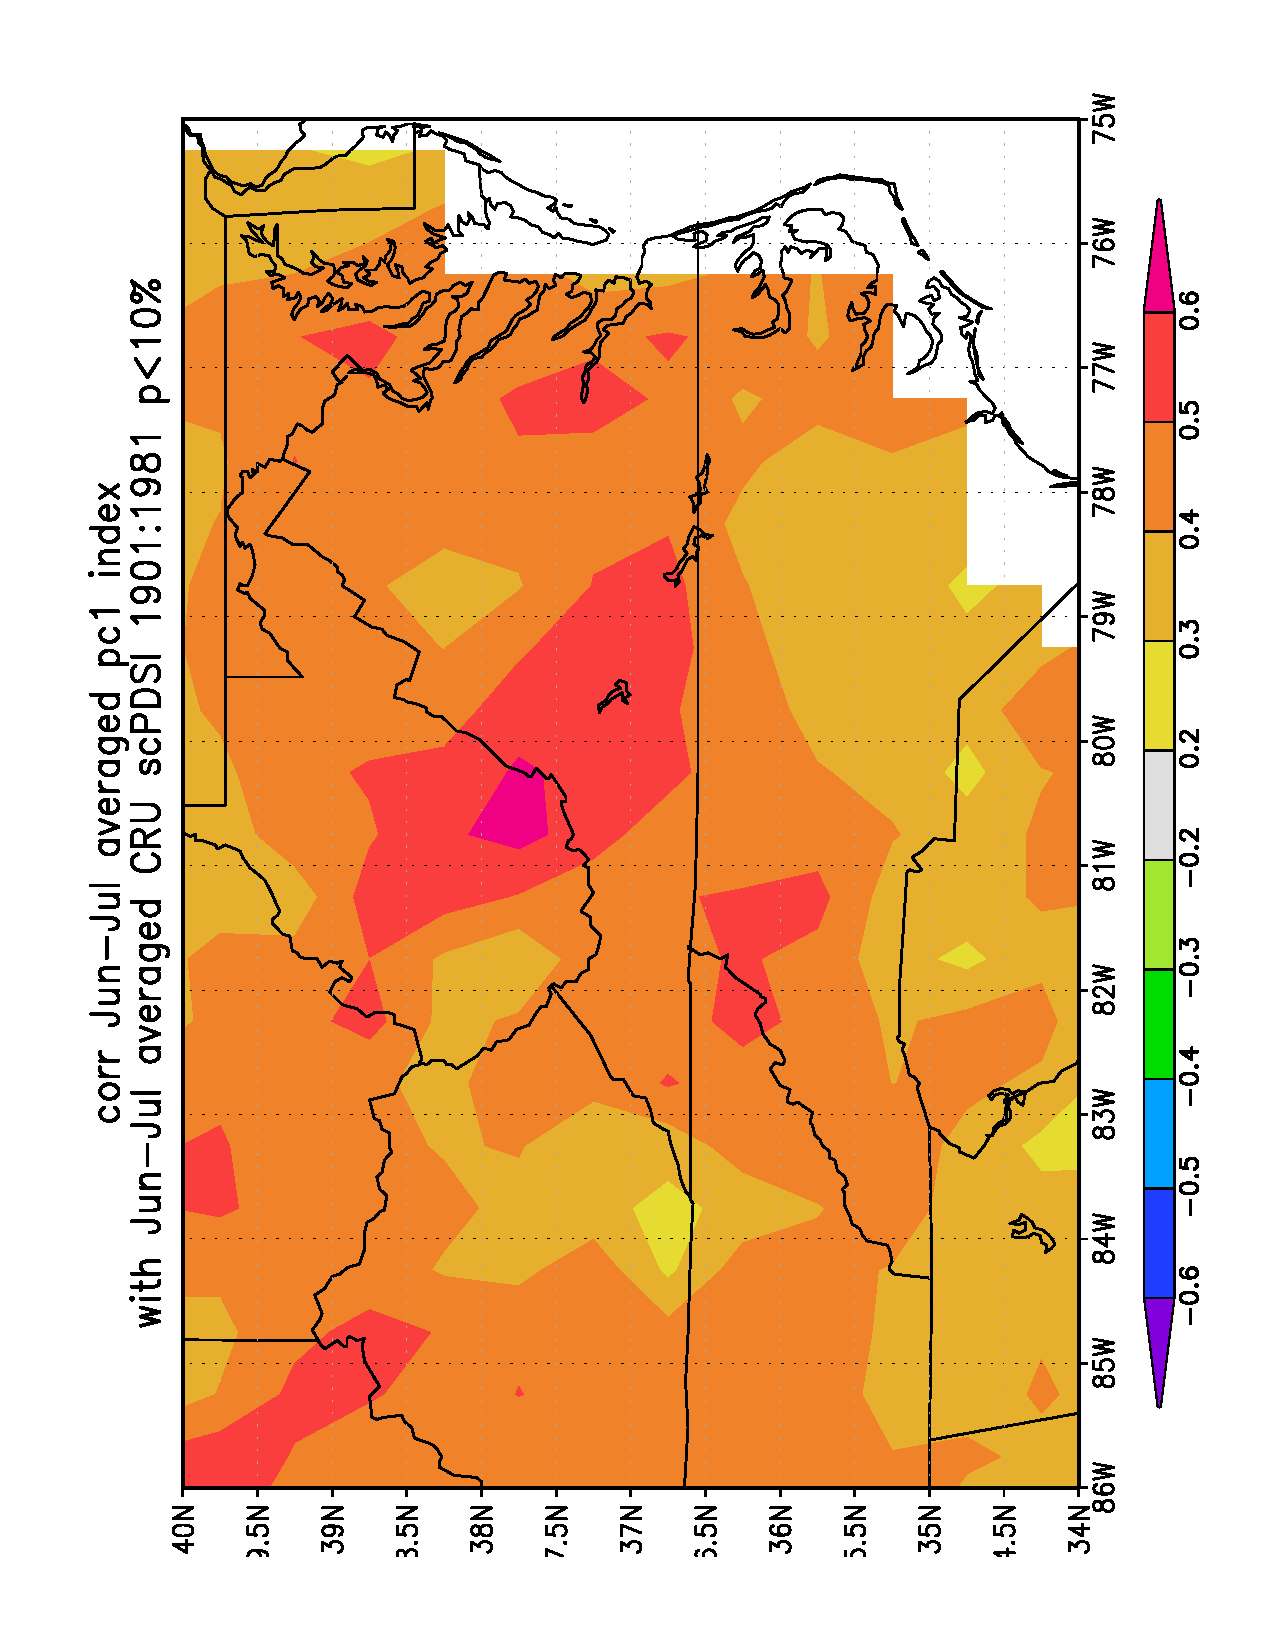
\includegraphics[width=5in, angle=-90]{figures/corrMapPdsiJJ.pdf}
%\caption{Correlation map.}
%\label{fig:pdsiCorrMap}
%\end{figure}
%
%\begin{figure}
%\centering
%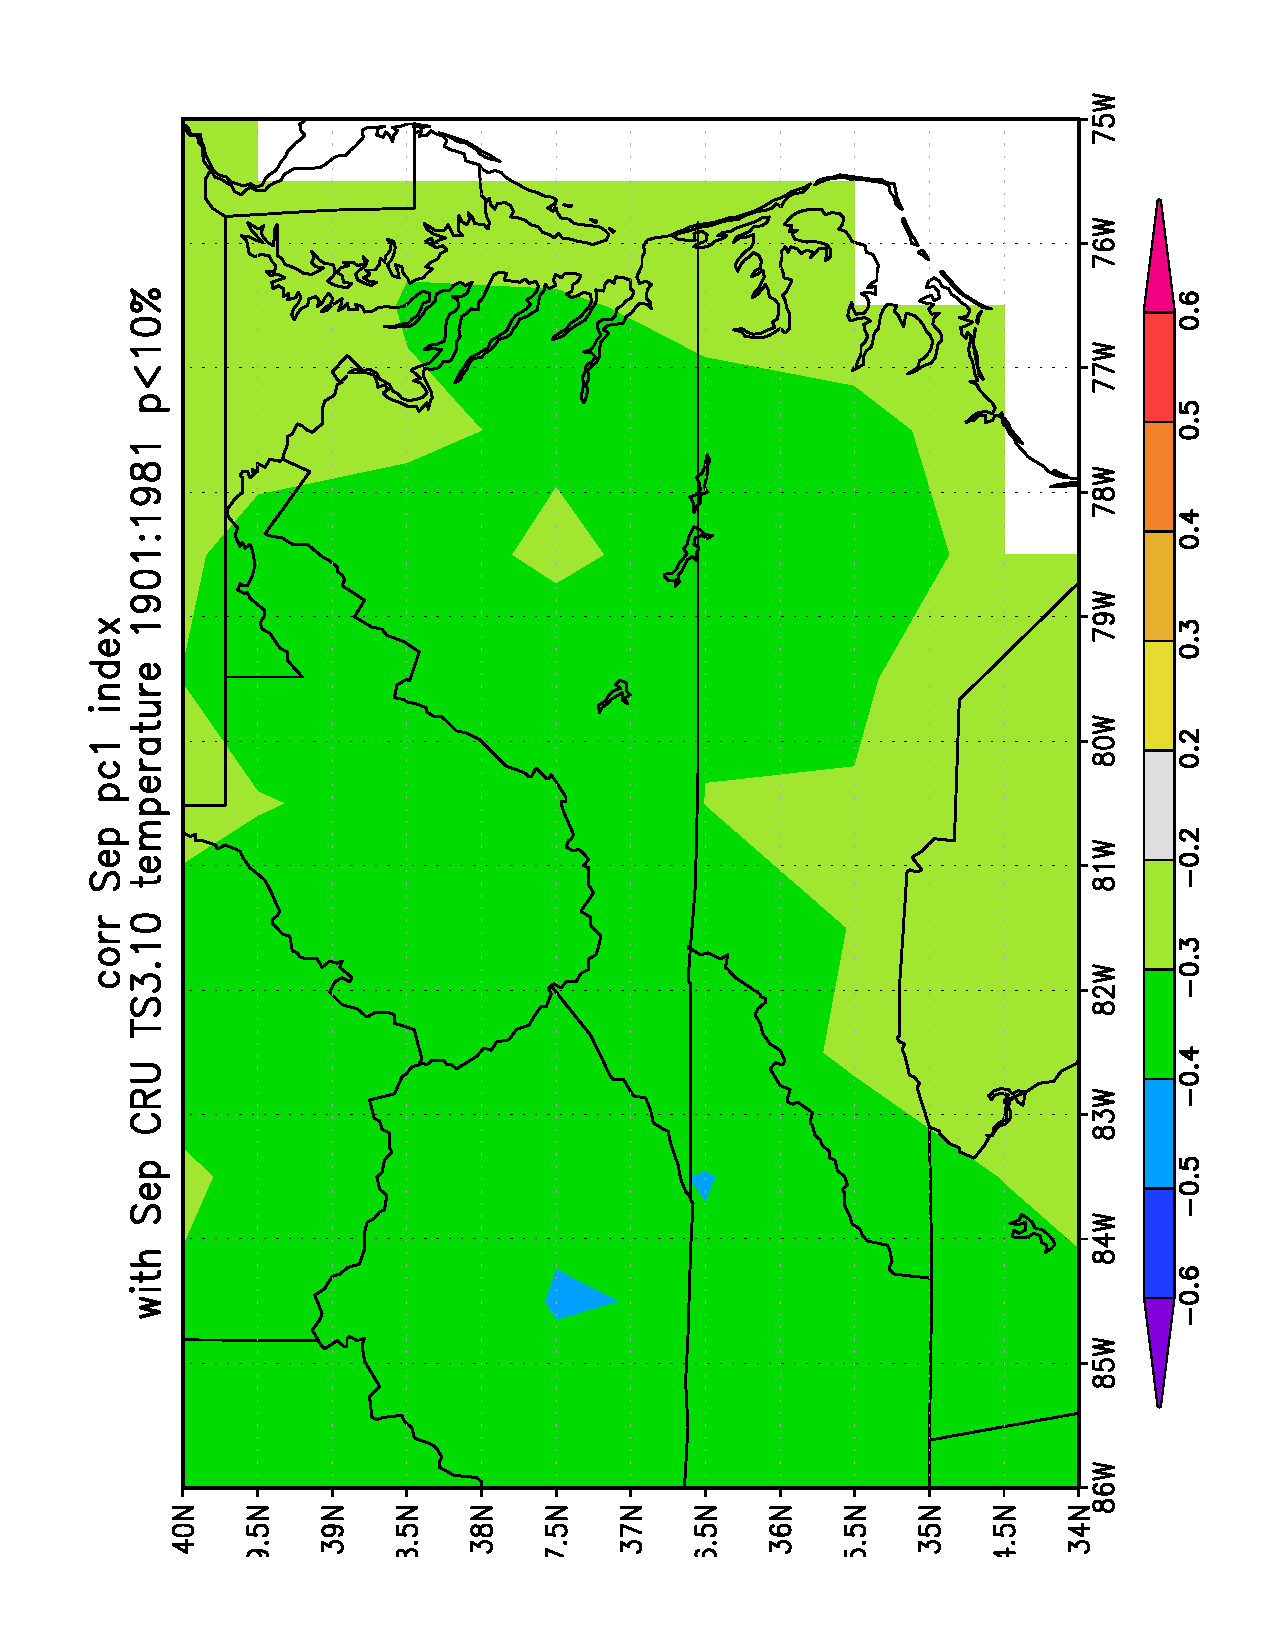
\includegraphics[width=5in, angle=-90]{figures/corrMapTempSept.pdf}
%\caption{Correlation map showing the correlation between the first principal component and September temperature.}
%\label{fig:tempCorrMap}
%\end{figure}

\begin{figure}
\centering
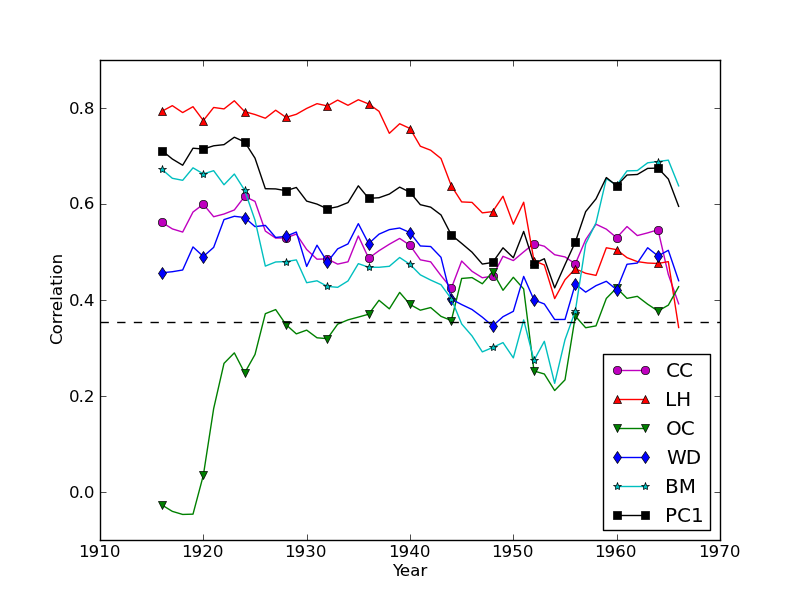
\includegraphics[width=5in]{figures/precipRunningCorr.png}
\caption{A 31-year windowed correlation plot showing the correlations between each growth proxy (chronologies and first principal component) and mjPR. Correlation points are plotted above the window centers.}
\label{fig:precipRunningCorr}
\end{figure}

\begin{figure}
\centering
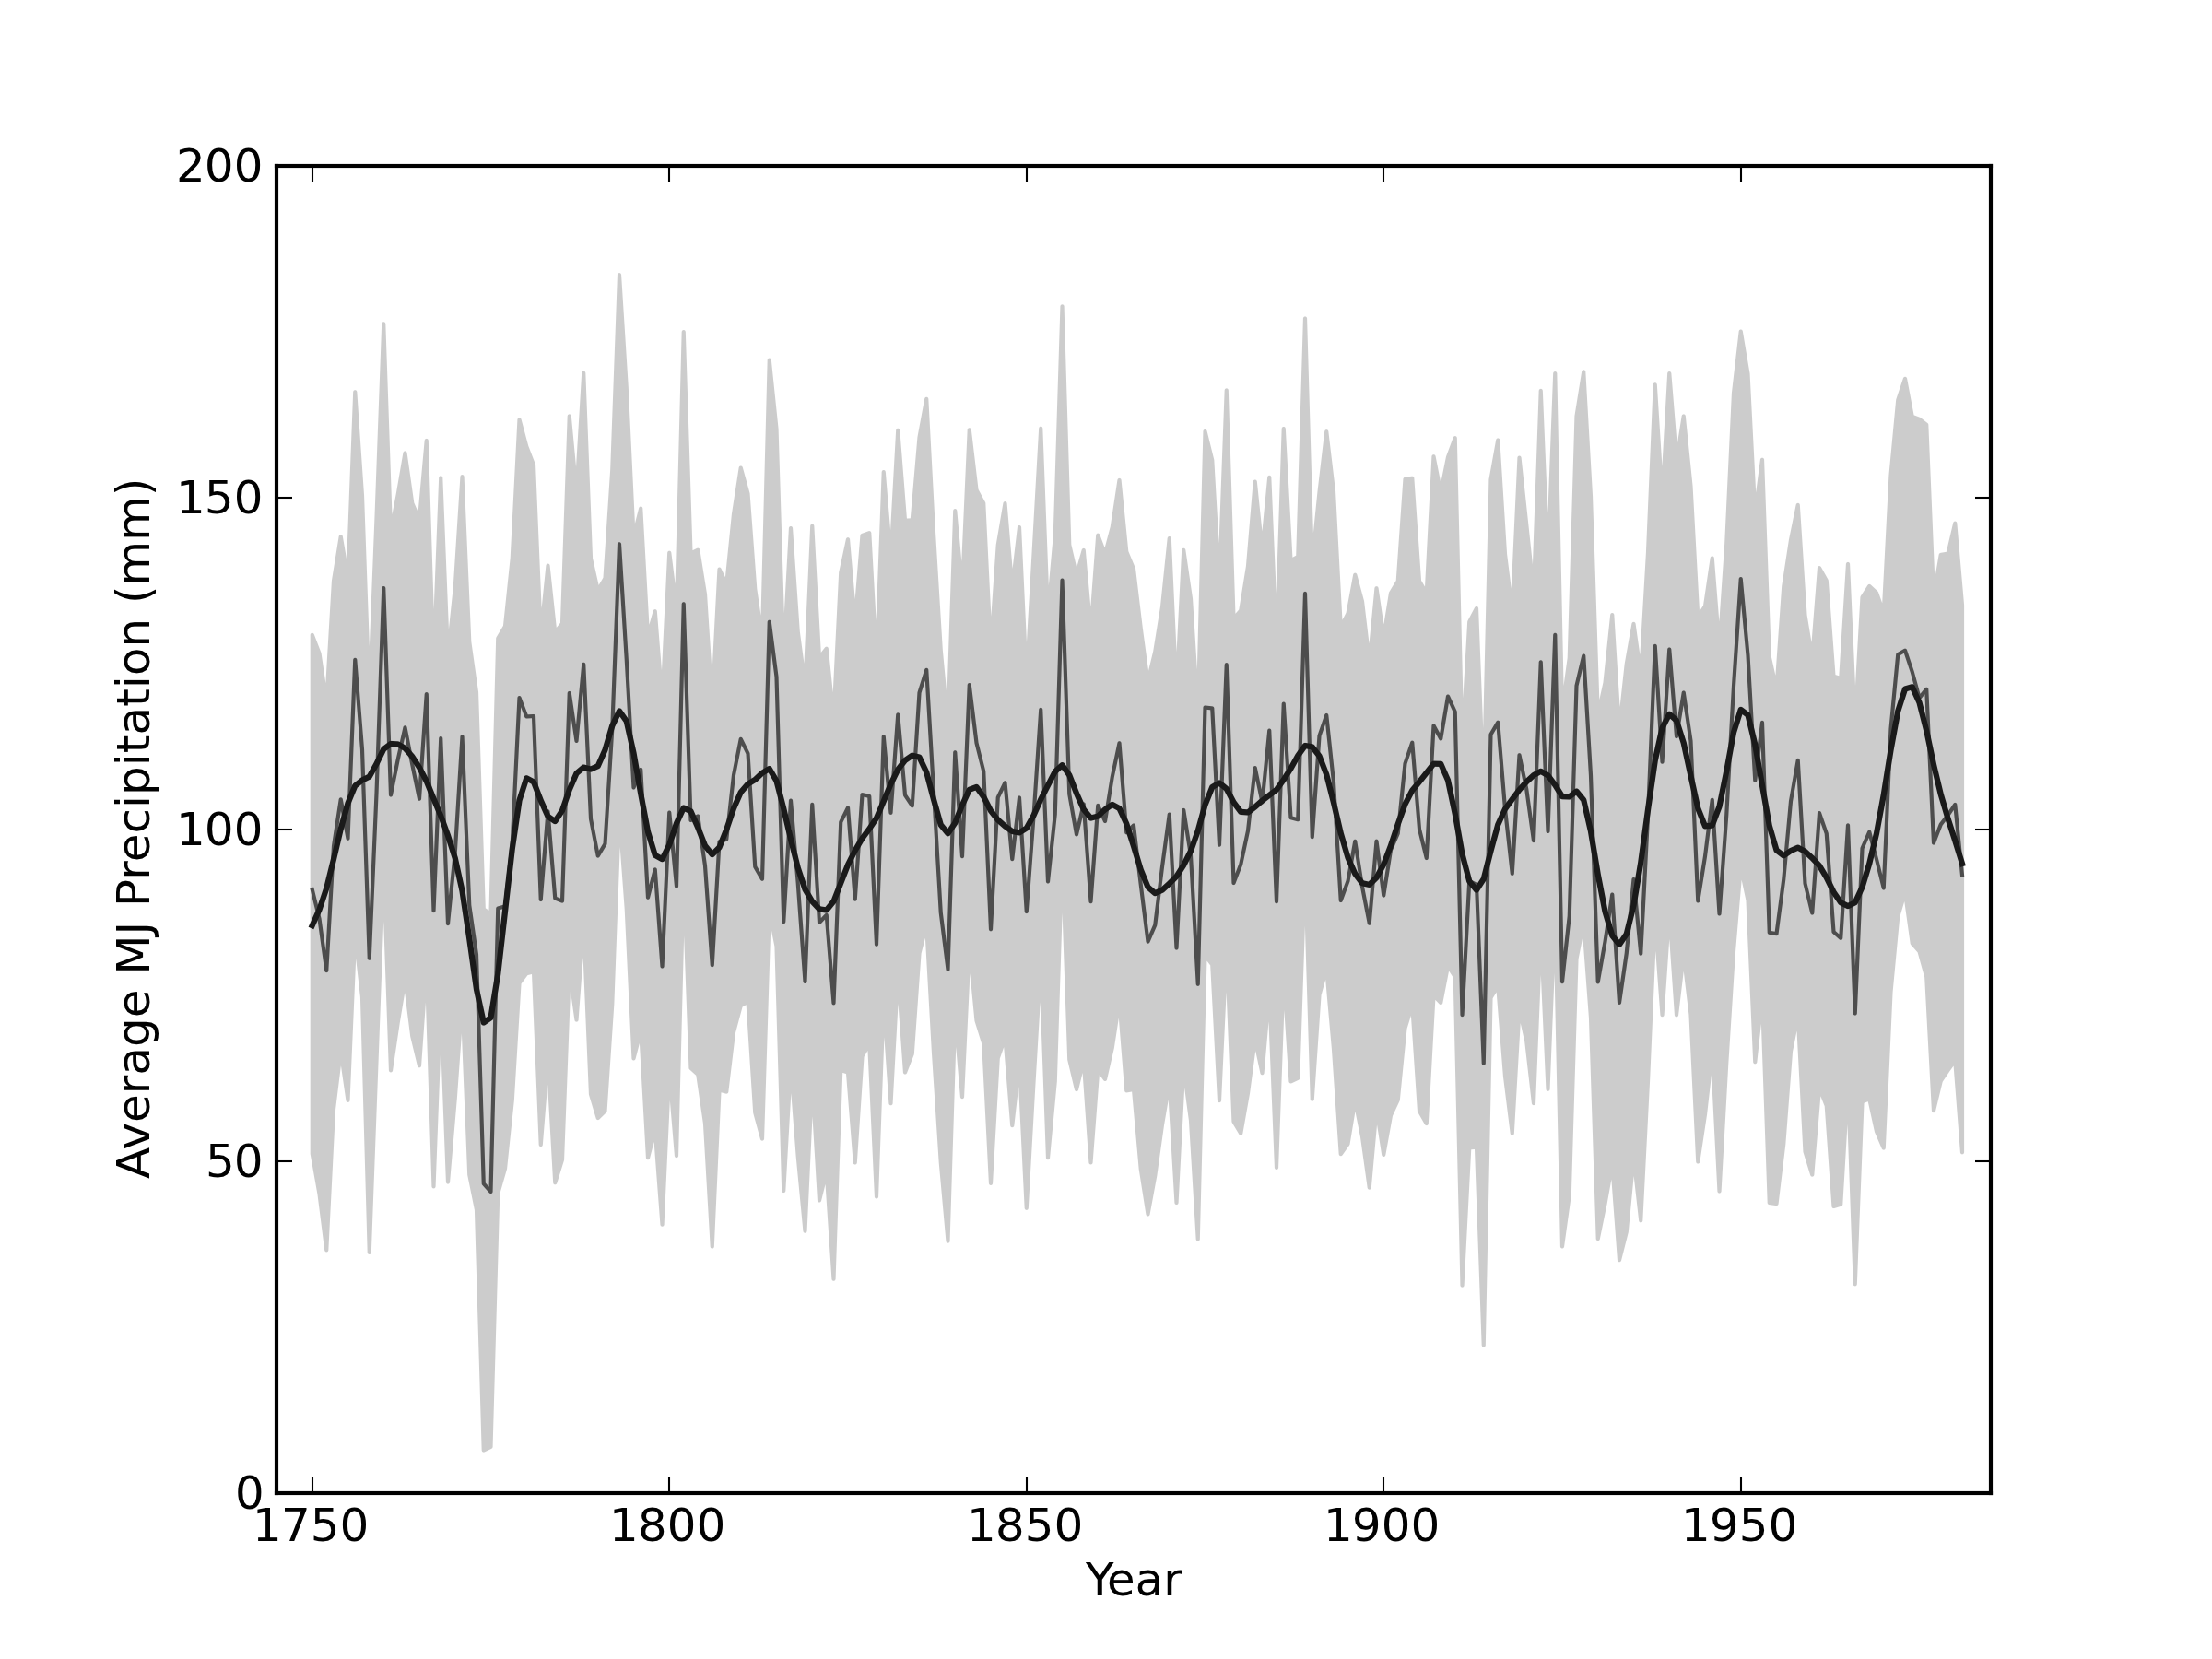
\includegraphics[width=5in]{figures/recon.png}
\caption{Average May-June precipitation (mjPR) reconstruction (grey curve), smoothed estimate showing decadal-scale variable (black curve), and the reconstruction 95\% credible interval (shaded grey region).}
\label{fig:precipRecon}
\end{figure}

\begin{figure}
\centering
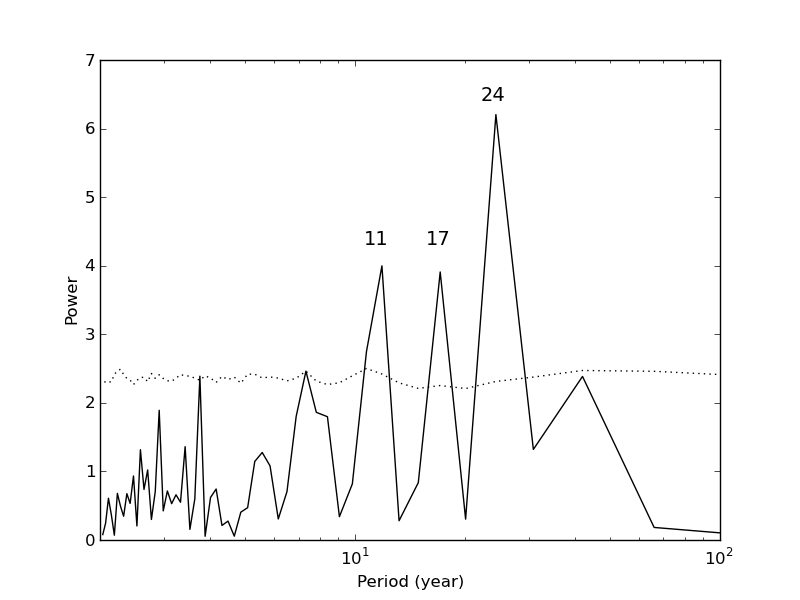
\includegraphics[width=5in]{figures/spectralRecon.png}
\caption{Periodogram showing periodicity of high amplitude at approximately 11, 17, and 24 years.}
\label{fig:spectral}
\end{figure}

\begin{figure}
\centering
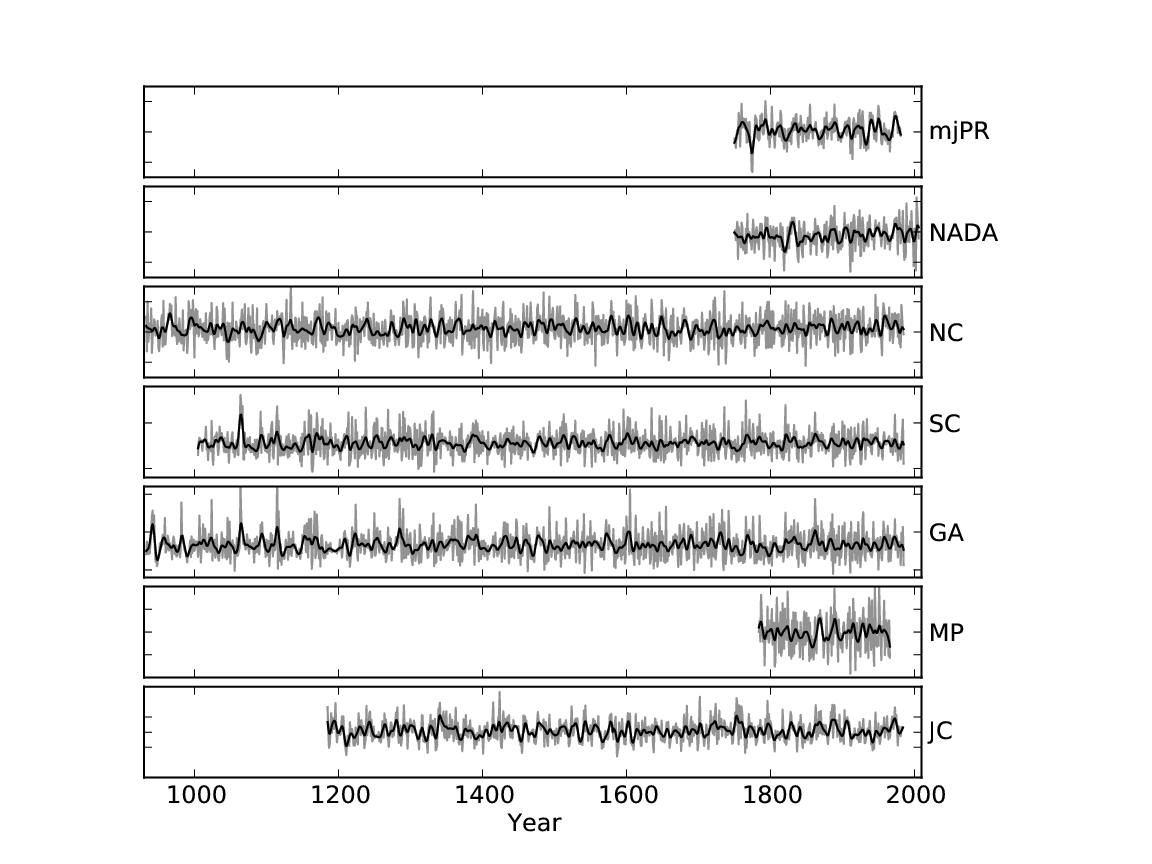
\includegraphics[width=5in]{figures/reconsStacked.png}
\caption{Time series plots showing annual- and decadal-scale variability for the mjPR and six compared moisture reconstructions for the period 933-2008.}
\label{fig:allRecons}
\end{figure}

\begin{figure}
\centering
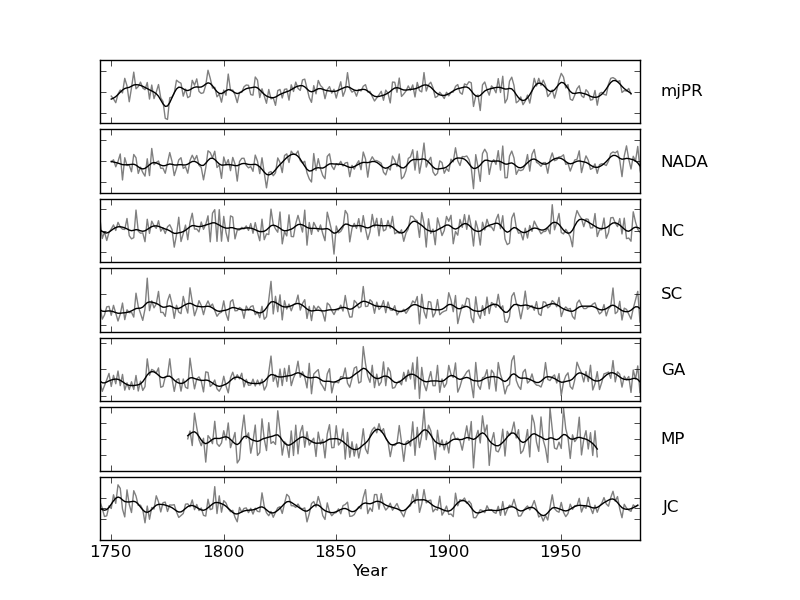
\includegraphics[width=5in]{figures/reconsStackedZoom.png}
\caption{Time series plots showing annual- and decadal-scale variability for the mjPR and six compared moisture reconstructions for the period 1745-1985.}
\label{fig:allReconsZoom}
\end{figure}


\begin{figure}
\centering
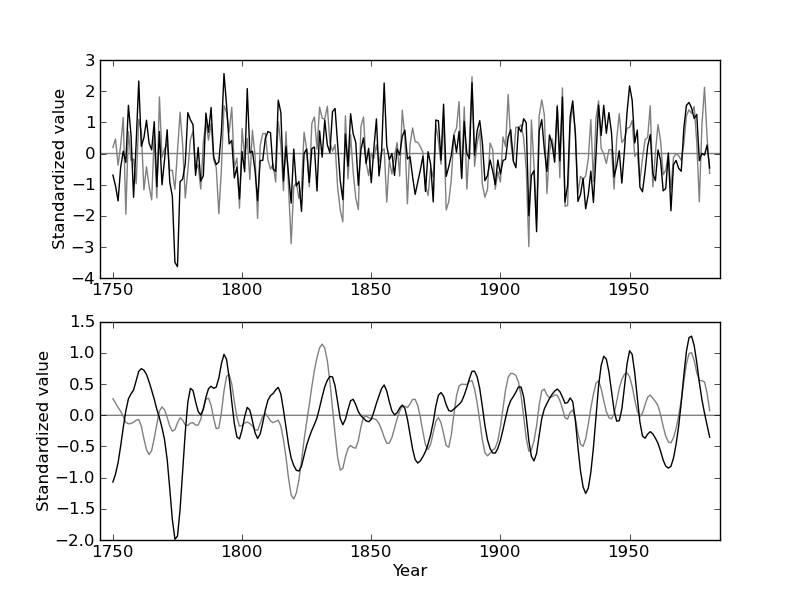
\includegraphics[width=5in]{figures/reconCompare.png}
\caption{Both the mjPR reconstruction and the Cook PDSI reconstruction are standardized and plotted against time to highlight both the similarities and the differences. Particularly notable differences include the year 1774, and the interval 1855-1863.}
\label{fig:reconCompare}
\end{figure}

\begin{figure}
\centering
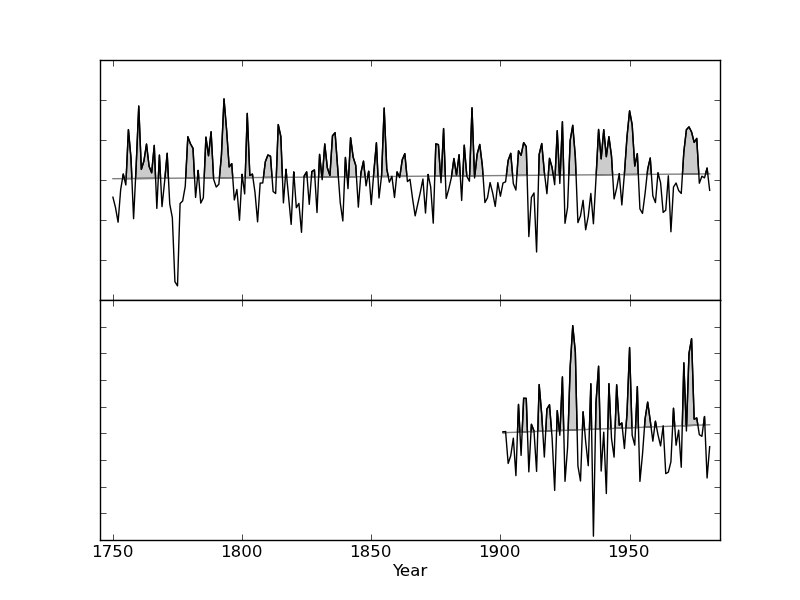
\includegraphics[width=5in]{figures/wetdry.png}
\caption{The mjPR reconstruction (top panel) and the mjPR instrumental record (bottom panel). Lines show the best-fit regression line through the time series data to indicate any dominant trends. Areas falling above the best-fit lines and the time series data are shaded grey to indicate periods of higher precipitation. Note the correspondence of wetter and drier years between the top and bottom panels.}
\label{fig:wetdry}
\end{figure}

\begin{figure}
\centering
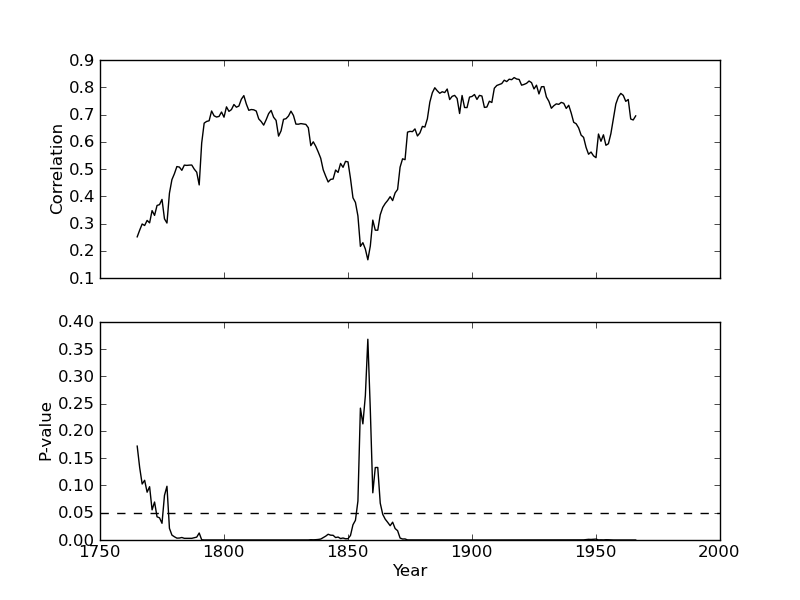
\includegraphics[width=5in]{figures/reconRunningCorr.png}
\caption{A 31 year windowed correlation plot between the mjPR and Cook PDSI reconstructions shows the discrepancy during the 1855-1863 interval. In the top panel correlation values are plotted about window centers, while the bottom panel shows the corresponding p-value (black) as well as the line of significance (dashed).}
\label{fig:reconRunningCorr}
\end{figure}

\begin{figure}
\centering
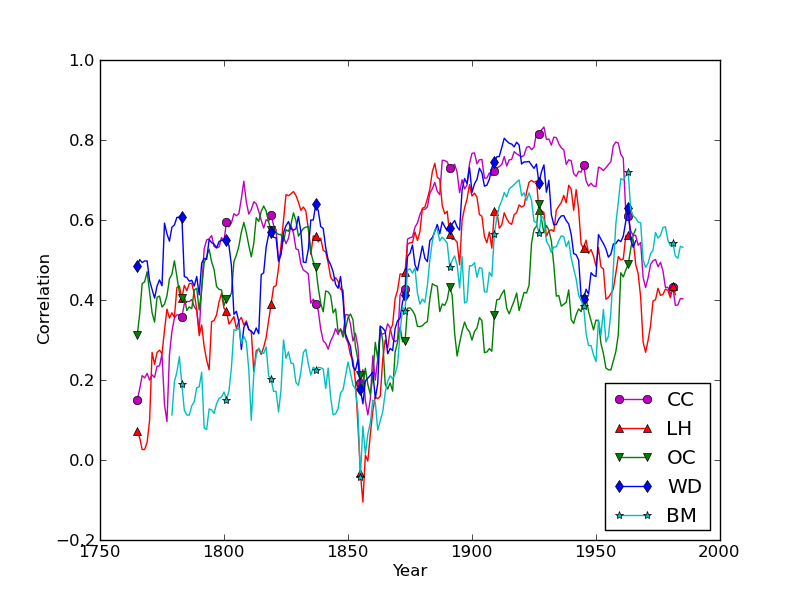
\includegraphics[width=5in]{figures/cookPdsiRunningCorr.png}
\caption{A 31 year windowed correlation plot between each of the chronologies and the Cook PDSI reconstruction. Note the interval of abrupt poor correlation during the years 1855-1863.}
\label{fig:cookRunningPdsiCorr}
\end{figure}



%%
%% reference
%%

\newpage
\clearpage
\bibliographystyle{unsrtnat}
\bibliography{oakRecon}

\end{document}
